\documentclass{article}
\usepackage[utf8]{inputenc}
\usepackage[a4paper, total={6.5in, 9.5in}]{geometry}
\usepackage{amscd}
\usepackage{amsfonts}
\usepackage{amsmath}
\usepackage{amssymb}
\usepackage{amsthm}
\usepackage{bbm}
\usepackage[makeroom]{cancel}
\usepackage{comment}
\usepackage{dashrule}
\usepackage{esint}
\usepackage{esvect}
\usepackage{fancyhdr}
\usepackage{graphicx, epsfig}
\usepackage{hyperref}
\usepackage{indentfirst}
\usepackage{latexsym}
%\usepackage{mathabx}
\usepackage{mathrsfs}
\usepackage{mathtools, nccmath}
\usepackage{parskip}
\usepackage{physics}
\usepackage{tcolorbox}
\usepackage{tikz-cd}
\usepackage{times} 
\usepackage{titlesec}
\usepackage{tocloft}
\usepackage{xcolor}
\usepackage{xy}

\setcounter{secnumdepth}{-2}

\makeatletter
\def\th@definition{\thm@notefont{}}
\makeatother

\let\qedsymbolclaim\qedsymbol

\theoremstyle{remark}
\newtheorem*{solution}{Solution}
\newenvironment{claimproof}{\begin{proof}[Proof of Claim]}{\end{proof}}

\theoremstyle{definition}
\newtheorem{theorem}{Theorem}[section]
\newtheorem{proposition}[theorem]{Proposition}
\newtheorem{lemma}[theorem]{Lemma}
\newtheorem{corollary}[theorem]{Corollary}
\newtheorem{conjecture}[theorem]{Conjecture}
\newtheorem{definition}[theorem]{Definition}
\newtheorem{remark}[theorem]{Remark}
\newtheorem*{claim}{Claim}
\newtheorem{example}[theorem]{Example}
\numberwithin{equation}{section}

\title{MATH 248 Tutorial Notes}
\author{Simon Chen and Ruth Wang}
\date{December 6, 2022}

\begin{document}

\maketitle

{
\centering \hypersetup{hidelinks}
\tableofcontents
}

\newpage 

\setcounter{section}{1}
\section{\centering Tutorial 1}

\subsection{Section 2.2}
\begin{tcolorbox}[
        title={Problem 8 (a)},
        valign=center,
        nobeforeafter,
        colframe=gray!95!black
    ]
Compute the following limit if it exists:
    \begin{align}
        \lim_{(x, y) \rightarrow (0, 0)} \frac{(x + y)^2 - (x - y)^2}{xy}
    \end{align}
\end{tcolorbox}

\begin{claim}
    The limit exists and is given by:
    \begin{align}
        \lim_{(x, y) \rightarrow (0, 0)} \frac{(x + y)^2 - (x - y)^2}{xy} &= 4
    \end{align}
\end{claim}

\begin{proof} We proceed by direct computation:
    \begin{align*}
        \lim_{(x, y) \rightarrow (0, 0)} \frac{(x + y)^2 - (x - y)^2}{xy} &= \lim_{(x, y) \rightarrow (0, 0)} \frac{\left(x^2 + 2xy + y^2\right) - \left(x^2 - 2xy + y^2\right)}{xy} \\
        &= \lim_{(x, y) \rightarrow (0, 0)} \frac{4xy}{xy} \\
        &= \lim_{(x, y) \rightarrow (0, 0)} 4 \\
        &= 4
    \end{align*}
\end{proof}

\begin{tcolorbox}[
        title={Problem 8 (b)},
        valign=center,
        nobeforeafter,
        colframe=gray!95!black
    ]
Compute the following limit if it exists:
    \begin{align}
        \lim_{(x, y) \rightarrow (0, 0)} \frac{\sin(xy)}{y}
    \end{align}
\end{tcolorbox}

\begin{claim}
    The limit exists and is given by:
    \begin{align}
        \lim_{(x, y) \rightarrow (0, 0)} \frac{\sin(xy)}{y} &= 0
    \end{align}
\end{claim}

\begin{proof}
\textit{(Taylor expansion)}

Observe that \(xy\) is small since \((x, y) \rightarrow (0, 0)\). 

Consider:
    \begin{align}
        \sin(t) &= t - \frac{t^3}{3!} + \frac{t^5}{5!} + ...
    \end{align}

\newpage 

Let \(t = xy\). This approximation is valid since \(xy\) is small Then:
    \begin{align*}
        \lim_{(x, y) \rightarrow (0, 0)} \frac{\sin(xy)}{y} &\approx \lim_{(x, y) \rightarrow (0, 0)} \frac{\left(xy - \frac{(xy)^3}{3!} + \frac{(xy)^5}{5!} + ...\right)}{y} \\
        &= \lim_{(x, y) \rightarrow (0, 0)} \frac{xy}{y} - \frac{(xy)^3}{3!y} + \frac{(xy)^5}{5!y} + ... \\
        &= \lim_{(x, y) \rightarrow (0, 0)} x - \frac{x^3y^2}{3!} + \frac{x^5y^4}{5!} + ... \\
        &= 0
    \end{align*}
\end{proof}

\begin{proof}
\textit{(\(\operatorname{sinc}\) function)}

Observe that \(xy\) is small since \((x, y) \rightarrow (0, 0)\). 

Recall from single variable calculus, proven by the Squeeze Theorem:
    \begin{align}
        \lim_{t \rightarrow 0} \frac{\sin(t)}{t} &= 1
    \end{align}

Let \(t = xy\). This approximation is valid since \(xy\) is small.

Then:
    \begin{align*}
        \lim_{(x, y) \rightarrow (0, 0)} \frac{\sin(xy)}{y} &= \lim_{(x, y) \rightarrow (0, 0)} x\frac{\sin(xy)}{xy} \\
        &= \lim_{(x, y) \rightarrow (0, 0)} x \cdot \lim_{(x, y) \rightarrow (0, 0)} \frac{\sin(xy)}{xy} \\
        &= 0 \cdot 1 \\
        &= 0
    \end{align*}
\end{proof}

\begin{tcolorbox}[
        title={Problem 26},
        valign=center,
        nobeforeafter,
        colframe=gray!95!black
    ]
Using either the \(\varepsilon - \delta\) definition of the limit or spherical coordinates, show that: 
    \begin{align}
        \lim_{(x, y, z) \rightarrow (0, 0, 0)} \frac{xyz}{x^2 + y^2 + z^2} &= 0
    \end{align}
\end{tcolorbox}

\begin{proof}
\textit{(\(\varepsilon - \delta\) definition)} 

Recall the \(\varepsilon - \delta\) definition of the limit. 

We say that \(\displaystyle \lim_{\vec{x} \rightarrow \vec{x}_0} f(\vec{x}) = L\) if for every \(\varepsilon > 0\), there exists a \(\delta > 0\) such that for all \((x, y, z)\):
\begin{align}
    \|\vec{x} - \vec{x}_0\| < \delta &\implies |f(\vec{x}) - L| < \varepsilon
\end{align}

In this problem, \(\vec{x}_0 = 0\) and \(L = 0\). We must show that for every \(\varepsilon > 0\), there exists a \(\delta > 0\) such that for all \((x, y, z)\):
\begin{align}
    \|\vec{x}\| < \delta &\implies |f(\vec{x}) - 0| < \varepsilon
\end{align}

Observe that, for all \(x\), \(y\), \(z \in \mathbb{R}\):
\begin{align}
    \left|\frac{x}{\sqrt{x^2 + y^2 + z^2}}\right| &\leq 1
\end{align}

Consider \(\delta = \varepsilon\):
\begin{align*}
    \left|\frac{xyz}{x^2 + y^2 + z^2} - 0\right| &= \left|\frac{xyz}{x^2 + y^2 + z^2}\right| \\
    &= \left|\frac{xyz}{x^2 + y^2 + z^2}\frac{\sqrt{x^2 + y^2 + z^2}}{\sqrt{x^2 + y^2 + z^2}}\right| \\
    &= \left|\frac{x}{\sqrt{x^2 + y^2 + z^2}}\frac{y}{\sqrt{x^2 + y^2 + z^2}}\frac{z}{\sqrt{x^2 + y^2 + z^2}}\sqrt{x^2 + y^2 + z^2}\right| \\
    &= \left|\frac{x}{\sqrt{x^2 + y^2 + z^2}}\right|\left|\frac{y}{\sqrt{x^2 + y^2 + z^2}}\right|\left|\frac{z}{\sqrt{x^2 + y^2 + z^2}}\right|\left|\sqrt{x^2 + y^2 + z^2}\right| \\
    &\leq 1 \cdot 1 \cdot 1 \cdot \left|\sqrt{x^2 + y^2 + z^2}\right| \\
    &= \left|\sqrt{x^2 + y^2 + z^2}\right| \\
    &= \|\vec{x}\| \\
    &< \delta \\
    &= \varepsilon
\end{align*}
\end{proof}

\begin{proof}
\textit{(Spherical coordinates)} 

Recall spherical coordinates:
\begin{align}
    x &= \rho \cos(\theta) \sin(\varphi) & y &= \rho \sin(\theta) \sin(\varphi) & z &= \rho \cos(\varphi) & \rho &= \sqrt{x^2 + y^2 + z^2}
\end{align}

Observe that, regardless of angle:
\begin{align}
    |\cos{(\theta)}| &\leq 1 & |\sin{(\theta)}| &\leq 1
\end{align}

Then:
\begin{align*}
    \left|\frac{xyz}{x^2 + y^2 + z^2}\right| &= \left|\frac{\rho \cos(\theta) \sin(\varphi)\rho \sin(\theta) \sin(\varphi)\rho \cos(\varphi)}{\rho^2}\right| \\
    &= \left|\rho \cos(\theta) \sin(\theta) \cos(\varphi) \sin^2(\varphi)\right| \\
    &= \left|\rho\right| \left|\cos(\theta)\right| \left|\sin(\theta)\right| \left|\cos(\varphi)\right| \left|\sin(\varphi)\right|^2 \\
    &\leq \left|\rho\right| 
\end{align*}

Since taking the limit as \((x, y, z) \rightarrow (0, 0, 0)\) is equivalent to shrinking the norm of the vector \((x, y, z)\) to zero, in spherical coordinates we will only be concerned with taking the limit as \(\rho \rightarrow 0\):
    \begin{align*}
        \lim_{(x, y, z) \rightarrow (0, 0, 0)} \left|\frac{xyz}{x^2 + y^2 + z^2}\right| &\leq \lim_{\rho \rightarrow 0} |\rho| \\
        &= 0
    \end{align*}
    
Therefore, by the Squeeze Theorem:
\begin{align}
        \lim_{(x, y, z) \rightarrow (0, 0, 0)} \frac{xyz}{x^2 + y^2 + z^2} &= 0
    \end{align}
\end{proof}

\subsection{Section 2.6}

\begin{tcolorbox}[
        title={Problem 16},
        valign=center,
        nobeforeafter,
        colframe=gray!95!black
    ]
Let \(f(x, y) = -\sqrt{1 - x^2 - y^2}\) for \((x, y)\) such that \(x^2 + y^2 < 1\). \\

Show that the plane tangent to the graph of \(f\) at \((x_0, y_0, f(x_0, y_0))\) is orthogonal to the vector with components \((x_0, y_0, f(x_0, y_0))\). Interpret this geometrically.
\end{tcolorbox}

\begin{proof}
    We first compute the partial derivatives of \(f\):
    \begin{align*}
        \frac{\partial f(x_0, y_0)}{\partial x} &= \frac{x}{\sqrt{1 - x^2 - y^2}}\Biggr|_{(x, y) = (x_0, y_0)} & \frac{\partial f(x_0, y_0)}{\partial y} &= \frac{y}{\sqrt{1 - x^2 - y^2}}\Biggr|_{(x, y) = (x_0, y_0)} \\
        &= \frac{x_0}{\sqrt{1 - x_0^2 - y_0^2}} & &= \frac{y_0}{\sqrt{1 - x_0^2 - y_0^2}}
    \end{align*}
    
    The equation of the plane tangent to the graph of \(f\) at \((x_0, y_0, f(x_0, y_0))\) is given by:
    \begin{align}
        z - f(x_0, y_0) &= \frac{\partial f(x_0, y_0)}{\partial x}(x - x_0) + \frac{\partial f(x_0, y_0)}{\partial y}(y - y_0)
    \end{align}
    
    The normal vector of this tangent plane is given by:
    \begin{align}
        \vec{n} &= \left(\frac{\partial f(x_0, y_0)}{\partial x}, \frac{\partial f(x_0, y_0)}{\partial y}, -1\right) \\
        &= \left(\frac{x_0}{\sqrt{1 - x_0^2 - y_0^2}}, \frac{y_0}{\sqrt{1 - x_0^2 - y_0^2}}, -1\right) 
    \end{align}
    
    In order to show that the plane tangent to the graph of \(f\) at \((x_0, y_0, f(x_0, y_0))\) is orthogonal to the vector with components \((x_0, y_0, f(x_0, y_0))\), it is sufficient to show that the normal vector of the tangent plane is parallel to the vector with components \((x_0, y_0, f(x_0, y_0))\).
    
    Equivalently, we want to show that there exists some constant \(k\) such that:
    \begin{align}
        k \vec{n} &= (x_0, y_0, f(x_0, y_0)) \\
        k \left(\frac{x_0}{\sqrt{1 - x_0^2 - y_0^2}}, \frac{y_0}{\sqrt{1 - x_0^2 - y_0^2}}, -1\right) &= \left(x_0, y_0, -\sqrt{1 - x_0^2 - y_0^2}\right) \\
        \left(\frac{kx_0}{\sqrt{1 - x_0^2 - y_0^2}}, \frac{ky_0}{\sqrt{1 - x_0^2 - y_0^2}}, -k\right) &= \left(x_0, y_0, -\sqrt{1 - x_0^2 - y_0^2}\right)
    \end{align}
    
    Then:
    \begin{align*}
        \begin{cases}
            \frac{kx_0}{\sqrt{1 - x_0^2 - y_0^2}} &= x_0 \\
            \frac{ky_0}{\sqrt{1 - x_0^2 - y_0^2}} &= y_0 \\
            -k &= -\sqrt{1 - x_0^2 - y_0^2}
        \end{cases} 
        &= 
        \begin{cases}
            kx_0 &= x_0 \sqrt{1 - x_0^2 - y_0^2} \\
            ky_0 &= y_0 \sqrt{1 - x_0^2 - y_0^2} \\
            k &= \sqrt{1 - x_0^2 - y_0^2}
        \end{cases} \\
        &= 
        \begin{cases}
            k &= \sqrt{1 - x_0^2 - y_0^2} \\
            k &= \sqrt{1 - x_0^2 - y_0^2} \\
            k &= \sqrt{1 - x_0^2 - y_0^2}
        \end{cases}
    \end{align*}
    
    Therefore, the plane tangent to the graph of \(f\) at \((x_0, y_0, f(x_0, y_0))\) is orthogonal to the vector with components \((x_0, y_0, f(x_0, y_0))\).
\end{proof}

\textit{Geometric interpretation.} Let \(f(x, y) = z\).

Observe that \(f\) is geometrically the southern hemisphere of the unit sphere:
\begin{align*}
    z &= -\sqrt{1 - x^2 - y^2} \\
    z^2 &= 1 - x^2 - y^2 \\
    x^2 + y^2 + z^2 &= 1
\end{align*}

Observe also that \((x_0, y_0, f(x_0, y_0)) = (x_0, y_0, z_0)\) is the position vector at the point \((x_0, y_0, z_0)\) on the sphere.

This implies that the plane tangent to any point on the southern hemisphere of the unit sphere is orthogonal to the position vector at that point. More generally, this is true for all spheres centered at the origin.

\begin{figure}[h!]
    \centering
    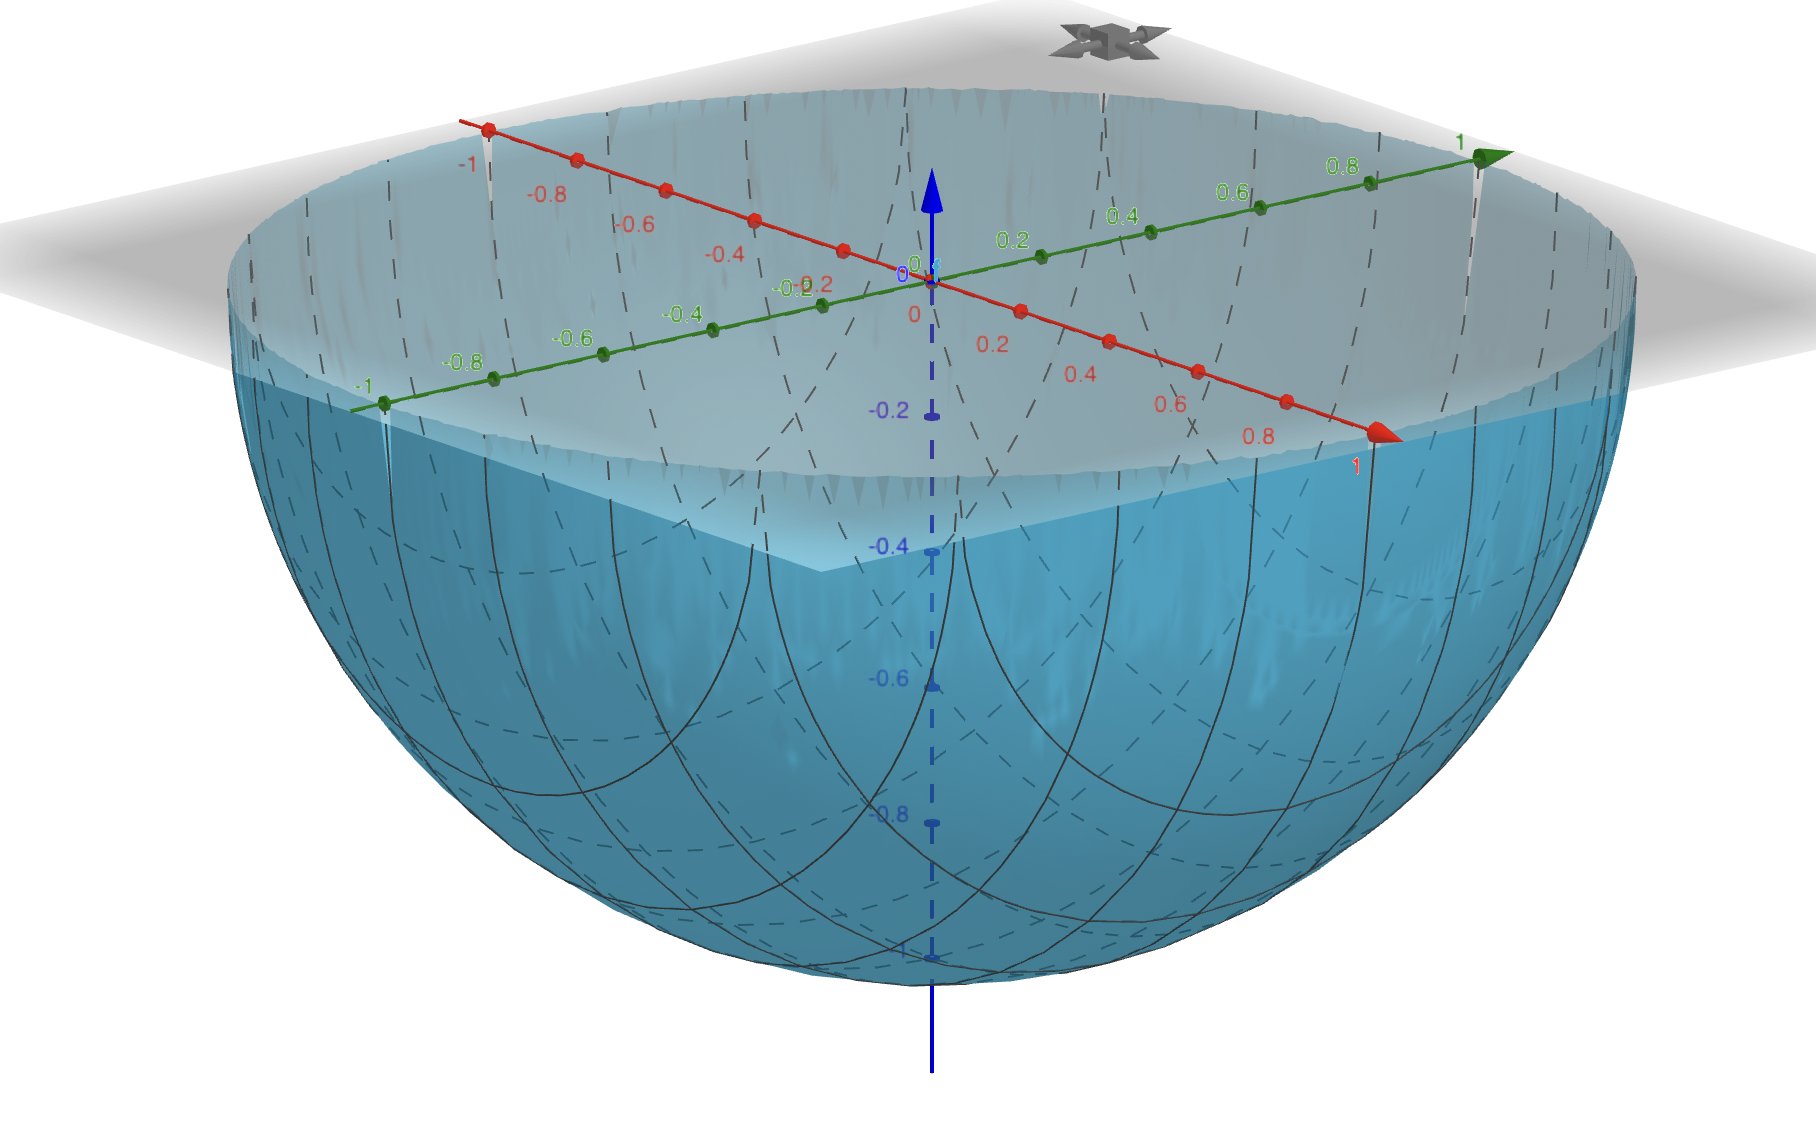
\includegraphics[width=15cm]{Pictures/Tutorial 1-1.png}
    \caption{Graph of \(f(x, y) = -\sqrt{1 - x^2 - y^2}\), which is the lower hemisphere of the unit sphere. Any position vector on the surface \((x,y,f(x,y))\) is normal to the surface.}
\end{figure}

\newpage

\setcounter{section}{2}
\section{\centering Tutorial 2}

\subsection{Section 2.5}

\begin{tcolorbox}[
        title={Problem 12},
        valign=center,
        nobeforeafter,
        colframe=gray!95!black
    ]
Let \(h: \mathbb{R}^3 \rightarrow \mathbb{R}^5\) and \(g: \mathbb{R}^2 \rightarrow \mathbb{R}^3\) be given by
\(h(x, y, z) = \left(xyz, e^{xz}, x \sin(y), -9x , 17\right)\) and \(g(u, v) = \left(v^2 + 2u, \pi, 2\sqrt{u}\right)\). \\

Find \(\vb{D}\left(h \circ g\right)(1, 1)\).
\end{tcolorbox}

\begin{solution}
    Observe that:
    \begin{align}
        g(1, 1) &= \left(1 + 2, \pi, 2\right) \\
        &= (3, \pi, 2)
    \end{align}
    
    Recall by the chain rule that:
    \begin{align}
        \vb{D}\left(h \circ g\right)(1, 1) &= \vb{D}h(3, \pi, 2) \vb{D}g(1, 1)
    \end{align}
    
    We compute the derivative matrices of \(h\) and \(g\):
    \begin{align*}
        \vb{D}\left(h\right)(x, y, z) &=
        \begin{bmatrix}
            yz & xz & xy \\
            ze^{xz} & 0 & xe^{xz} \\
            \sin{(y)} & x\cos{(y)} & 0 \\
            \frac{9}{x^2} & 0 & 0 \\
            0 & 0 & 0
        \end{bmatrix} & \vb{D}\left(g\right)(u, v) &=
        \begin{bmatrix}
            2 & 2v \\
            0 & 0 \\
            \frac{1}{\sqrt{u}} & 0
        \end{bmatrix}
    \end{align*}
    
    Then:
    \begin{align*}
        \vb{D}\left(h \circ g\right)(1, 1) &= \vb{D}h(3, \pi, 2) \vb{D}g(1, 1) \\
        &= 
        \begin{bmatrix}
            2\pi & 6 & 3\pi \\
            2e^6 & 0 & 3e^6 \\
            \sin{(\pi)} & 3\cos{(\pi)} & 0 \\
            \frac{9}{3^2} & 0 & 0 \\
            0 & 0 & 0
        \end{bmatrix}
        \begin{bmatrix}
            2 & 2 \\
            0 & 0 \\
            \frac{1}{\sqrt{1}} & 0
        \end{bmatrix} \\
        &= 
        \begin{bmatrix}
            2\pi & 6 & 3\pi \\
            2e^6 & 0 & 3e^6 \\
            0 & -3 & 0 \\
            1 & 0 & 0 \\
            0 & 0 & 0
        \end{bmatrix}
        \begin{bmatrix}
            2 & 2 \\
            0 & 0 \\
            1 & 0
        \end{bmatrix} \\
        &= 
        \begin{bmatrix}
            4\pi + 3\pi & 4\pi \\
            4e^6 + 3e^6 & 4^6 \\
            0 & 0 \\
            2 & 2 \\
            0 & 0
        \end{bmatrix} \\
        &= 
        \begin{bmatrix}
            7\pi & 4\pi \\
            7e^6 & 4^6 \\
            0 & 0 \\
            2 & 2 \\
            0 & 0
        \end{bmatrix}
    \end{align*}
\end{solution}

\subsection{Section 2.6}

\begin{tcolorbox}[
        title={Problem 22 (a)},
        valign=center,
        nobeforeafter,
        colframe=gray!95!black
    ]
Captain Ralph is in trouble near the sunny side of Mercury. The temperature of the ship's hull when he is at location \((x, y, z)\) will be given by \(T(x, y, z) = e^{-x^2 - 2y^2 - 3z^2}\), where \(x\), \(y\), and \(z\) are measured in meters. He is currently at \((1, 1, 1)\). \\

In what direction should he proceed in order to
decrease the temperature most rapidly?
\end{tcolorbox}

\begin{solution}
    Recall that the direction of the gradient is the direction of maximal increase.
    
    The direction of maximal decrease is therefore the direction of the negative of the gradient.
    
    We first compute the gradient of \(T\):
    \begin{align}
        \nabla T(x, y, z) &= \left(-2xe^{-x^2 - 2y^2 - 3z^2}, -4ye^{-x^2 - 2y^2 - 3z^2}, -6ze^{-x^2 - 2y^2 - 3z^2}\right)
    \end{align}
    
    The direction of maximal decrease at \((1, 1, 1)\) is therefore given by:
    \begin{align*}
        -\nabla T(1, 1, 1) &= -\left(-2e^{-1 - 2 - 3}, -4e^{-1 - 2 - 3}, -6e^{-1 - 2 - 3}\right) \\
        &= -\left(-2e^{-6}, -4e^{-6}, -6e^{-6}\right) \\
        &= \left(2, 4, 6\right)e^{-6}
    \end{align*}
    
    The direction of maximal decrease is given by the vector \((2, 4, 6)\). You may normalize the vector if you wish, but it is not necessary.
\end{solution}

\begin{tcolorbox}[
        title={Problem 22 (b)},
        valign=center,
        nobeforeafter,
        colframe=gray!95!black
    ]
If the ship travels at \(e^8\) meters per second, how fast
will be the temperature decrease if he proceeds in
that direction?
\end{tcolorbox}

\begin{solution}
    Let \(\vec{v}\) be the velocity of the ship. The rate of change of the temperature along \(\vec{u}\) is given by the directional derivative:
    \begin{align}
        \vec{u} \cdot \nabla T
    \end{align}
    
    We note that \(\vec{u}\) is in the direction of \(-\nabla T\) and that \(\|\vec{u}\| = e^8\). 
    
    Then:
    \begin{align*}
        \vec{u} \cdot \nabla T &= \|\vec{u}\|\|\nabla T\| \cos(\pi) \\
        &= e^8\sqrt{2^2 + 4^2 + 6^2}e^{-6} \cos(\pi) \\
        &= -\sqrt{56}e^2 \\
        &= - 2\sqrt{14}e^2
    \end{align*}
    
    Note that the \(\cos(\pi)\) results from the fact that \(\vec{u}\) and \(\nabla T\) point in opposite directions. 
    
    For those who wish to be more rigorous, we may have written:
    \begin{align}
        \vec{u} &= -\frac{\nabla T}{\|\nabla T\|}\|\vec{u}\| \\
        &= -\frac{\nabla T}{\|\nabla T\|}e^8
    \end{align}
    since \(e^8\) is the magnitude of \(\vec{u}\) and \(-\frac{\nabla T}{\|\nabla T\|}\) is the unit direction vector of \(\vec{u}\). 
    
    The directional derivative therefore becomes:
    \begin{align*}
        \vec{u} \cdot \nabla T &= -\frac{\nabla T}{\|\nabla T\|}e^8 \cdot \nabla T \\
        &= -\frac{\|\nabla T\|^2}{\|\nabla T\|}e^8 \\
        &= -\|\nabla T\| e^8 \\
        &= -\sqrt{2^2 + 4^2 + 6^2} e^{-6} e^8 \\
        &= -\sqrt{56}e^2 \\
        &= - 2\sqrt{14}e^2
    \end{align*}
    
    Either way, the temperature decreases at a rate of \(2\sqrt{14}e^2\) degrees per second.
\end{solution}

\begin{tcolorbox}[
        title={Problem 22 (c)},
        valign=center,
        nobeforeafter,
        colframe=gray!95!black
    ]
Unfortunately, the metal of the hull will crack if
cooled at a rate greater than \(\sqrt{14}e^2\) degrees per
second. Describe the set of possible directions in
which he may proceed to bring the temperature
down at no more than that rate.
\end{tcolorbox}

\begin{solution}
    Since we cannot cool the hull faster than \(\sqrt{14}e^2\) degrees per second, we impose the following condition:
    \begin{align}
        -\sqrt{14}e^2 &\leq \vec{u} \cdot \nabla T
    \end{align}
    
    We compute the directional derivative:
    \begin{align*}
        \vec{u} \cdot \nabla T &= \|\vec{u}\|\|\vec{T}\| \cos(\theta) \\
        &= 2e^8\sqrt{14} e^{-6} \cos(\theta) \\
        &= 2\sqrt{14} e^{2} \cos(\theta)
    \end{align*}
    
    This condition is satisfied when:
    \begin{align*}
        -\sqrt{14}e^2 &\leq 2\sqrt{14} e^{2} \cos(\theta) \\
        -1 &\leq 2 \cos(\theta) \\
        -\frac{1}{2} &\leq \cos(\theta)
    \end{align*}
    
    This implies that \(\theta \in \left[0, \frac{2\pi}{3}\right] \cup \left[\frac{4\pi}{3}, 2\pi\right]\).
    
    Depending on your interpretation of this question, if we want to further restrict the angle by considering only directions in which the temperature decreases, we impose the next condition:
    \begin{align}
        \vec{u} \cdot \nabla T &< 0 
    \end{align}
    
    This condition is satisfied when:
    \begin{align*}
        2\sqrt{14} e^{2} \cos(\theta) &< 0 \\
        \cos(\theta) &< 0
    \end{align*}
    
    This implies that \(\theta \in \left(\frac{\pi}{2}, \frac{3\pi}{2}\right)\).
    
    If we want to bring the temperature down without cooling it too fast, both of these conditions must hold simultaneously. We therefore have that \(\theta \in \left(\frac{\pi}{2}, \frac{2\pi}{3}\right] \cup \left[\frac{4\pi}{3}, \frac{3\pi}{2}\right)\).
    
    We recommend you draw a unit circle if this does not convince you.
\end{solution}

\subsection{Section 3.1}

\begin{tcolorbox}[
        title={Problem 22},
        valign=center,
        nobeforeafter,
        colframe=gray!95!black
    ]
Let \(w = f(x, y)\) be a \(C^2\) function of two variables and let \(x = u + v\), \(y = u - v\). \\

Show that:
\begin{align}
    \frac{\partial^2 w}{\partial u \partial v} &= \frac{\partial^2 w}{\partial x^2} - \frac{\partial^2 w}{\partial y^2}
\end{align}
\end{tcolorbox}

\begin{proof}
    We first compute the partial derivatives of \(x\) and \(y\):
    \begin{align}
        \frac{\partial x}{\partial u} &= 1 & \frac{\partial x}{\partial v} &= 1 \\
        \frac{\partial y}{\partial u} &= 1 & \frac{\partial y}{\partial v} &= -1
    \end{align}
    
    By the chain rule:
    \begin{align*}
        \frac{\partial w}{\partial v} &= \frac{\partial w}{\partial x}\frac{\partial x}{\partial v} + \frac{\partial w}{\partial y}\frac{\partial y}{\partial v} \\
        &= \frac{\partial w}{\partial x}\cancelto{1}{\frac{\partial x}{\partial v}} + \frac{\partial w}{\partial y}\cancelto{-1}{\frac{\partial y}{\partial v}} \\
        &= \frac{\partial w}{\partial x} - \frac{\partial w}{\partial y} \\
        &= w_x - w_y
    \end{align*}
    
    And:
    \begin{align*}
        \frac{\partial^2 w}{\partial u \partial v} &= \frac{\partial w_x}{\partial u} - \frac{\partial w_y}{\partial u} \\
        &= \frac{\partial w_x}{\partial x}\frac{\partial x}{\partial u} + \frac{\partial w_x}{\partial y}\frac{\partial y}{\partial u} - \frac{\partial w_y}{\partial x}\frac{\partial x}{\partial u} - \frac{\partial w_y}{\partial y}\frac{\partial y}{\partial u} \\
        &= \frac{\partial w_x}{\partial x}\cancelto{1}{\frac{\partial x}{\partial u}} + \frac{\partial w_x}{\partial y}\cancelto{1}{\frac{\partial y}{\partial u}} - \frac{\partial w_y}{\partial x}\cancelto{1}{\frac{\partial x}{\partial u}} - \frac{\partial w_y}{\partial y}\cancelto{1}{\frac{\partial y}{\partial u}} \\
        &= \frac{\partial w_x}{\partial x} + \frac{\partial w_x}{\partial y} - \frac{\partial w_y}{\partial x} - \frac{\partial w_y}{\partial y} \\
        &= \frac{\partial^2 w}{\partial x^2} + \frac{\partial^2 w}{\partial y \partial x} - \frac{\partial^2 w}{\partial x \partial y} - \frac{\partial^2 w}{\partial y^2} \\
        &= \frac{\partial^2 w}{\partial x^2} + \frac{\partial^2 w}{\partial y \partial x} - \frac{\partial^2 w}{\partial y \partial x} - \frac{\partial^2 w}{\partial y^2} \\
        &= \frac{\partial^2 w}{\partial x^2} - \frac{\partial^2 w}{\partial y^2} 
    \end{align*}
\end{proof}

\newpage 

\setcounter{section}{3}
\section{\centering Tutorial 3}

\subsection{Section 3.3}

\begin{tcolorbox}[
        title={Problem 24},
        valign=center,
        nobeforeafter,
        colframe=gray!95!black
    ]
Let \(f(x, y) = Ax^2 + B\), where \(A\) and \(B\) are constants. \\

What are the critical points of \(f\)? Are they local maxima or local minima?
\end{tcolorbox}

\begin{solution}
    We first compute the gradient of \(f\):
    \begin{align}
        \nabla f(x, y) &= \left(2Ax, 0\right)
    \end{align}
    
    The gradient is equal to \((0, 0)\) when \((x, y) = (0, y)\) where \(y\) is allowed to vary.
    
    The critical points of \(f\) are all the points along the \(y\)-axis.
    
    Recall one definition of local extrema:
    \begin{itemize}
        \item \((x_0, y_0)\) is a local minimum if the Hessian \(H_f(x_0, y_0)\) is positive semidefinite.
        \item \((x_0, y_0)\) is a local maximum if the Hessian \(H_f(x_0, y_0)\) is negative semidefinite.
    \end{itemize}
    
    Recall also the definition of positive and negative semidefinite:
    \begin{itemize}
        \item A \(2 \times 2\) or \(3 \times 3\) matrix \(A\) is positive definite if \(a_{11} > 0\) and \(\det(A) > 0\)
        \item A \(2 \times 2\) or \(3 \times 3\) matrix \(A\) is negative definite if \(a_{11} < 0\) and \(\det(A) < 0\)
    \end{itemize}
    
    We now compute the Hessian matrix of \(f\):
    \begin{align*}
        H_f(0, y) &= 
        \begin{pmatrix}
            \frac{\partial^2 f}{\partial x^2} & \frac{\partial^2 f}{\partial y \partial x} \\
            \frac{\partial^2 f}{\partial x \partial y} & \frac{\partial^2 f}{\partial y^2} 
        \end{pmatrix} \\
        &= 
        \begin{pmatrix}
            \frac{\partial}{\partial x}(2Ax) & \frac{\partial}{\partial y}(2Ax) \\
            \frac{\partial}{\partial x}(0) & \frac{\partial}{\partial y}(0)
        \end{pmatrix} \\
        &= 
        \begin{pmatrix}
            2A & 0 \\
            0 & 0
        \end{pmatrix}
    \end{align*}
    
    We now compute the determinant:
    \begin{align}
        \det\left(H_f(0, y)\right) &= 2A(0) - 0 \\
        &= 0
    \end{align}
    
    Unfortunately we cannot gather any information since \(\det\left(H_f(0, y)\right) = 0\). We therefore proceed by inspection.
    
    Observe that \(f(x, y)\) does not actually depend on \(y\). We fix some arbitrary \(y = y_0\). Then \(f(x, y) = f(x)\).
    
    From single variable calculus, the concavity of a function \(f\) is determined by the second derivative of \(f\):
    \begin{align*}
        f''(x) &= (Ax^2 + B)'' \\
        &= (2Ax)' \\
        &= 2A
    \end{align*}
    
    Then \(x = 0\) is a local minimum if \(A > 0\) and \(x = 0\) is a local maximum if \(A < 0\).
    
    Similarly, \((x, y) = (0, y)\) are local minima if \(A > 0\) and \((0, y) = (0, y)\) are local maxima if \(A < 0\).
\end{solution}

\begin{tcolorbox}[
        title={Problem 44},
        valign=center,
        nobeforeafter,
        colframe=gray!95!black
    ]
Let \(f(x, y) = 1 + xy + x - 2y\) and let \(D\) be the triangular region in \(\mathbb{R}^2\) with vertices \((1, -2)\), \((5, -2)\), and \((1, 2)\). \\

Find the absolute maximum and minimum values of \(f\) on \(D\). Give all points where these extreme values occur.
\end{tcolorbox}

\begin{solution}
    We first compute the gradient of \(f\):
    \begin{align}
        \nabla f(x, y) &= \left(y + 1, x - 2\right)
    \end{align}
    
    The gradient is equal to \((0, 0)\) when \((x, y) = (2, -1)\).
    
    The only critical point of \(f\) in \(D\) is \((x, y) = (2, -1)\).
    
    We now proceed to find all extrema of \(f\) on the boundary.
    
    \begin{figure}[h]
        \centering
        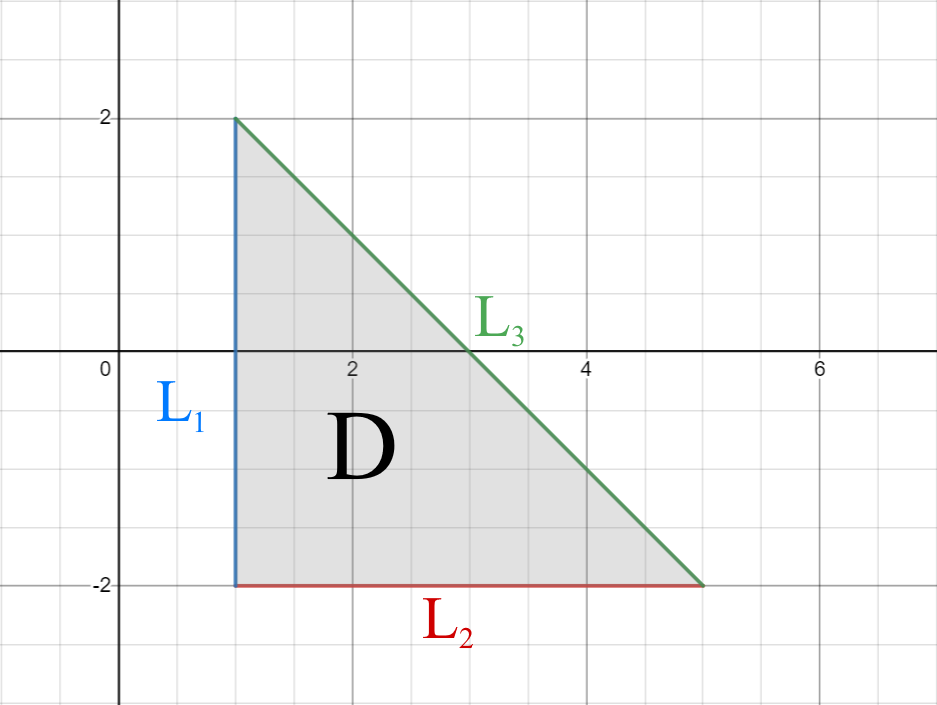
\includegraphics[width=0.4\textwidth]{Pictures/Tutorial 3-1.png}
        \caption{Triangular region in \(\mathbb{R}^2\) with vertices \((1, -2)\), \((5, -2)\), and \((1, 2)\).}
    \end{figure}
    
    On the curve \(L_1\), we have \(x = 1\) and \(-2 \leq y \leq 2\). 
    
    Then:
    \begin{align*}
        f(1, y) &= 1 + y + 1 - 2y \\
        &= 2 - y
    \end{align*}
    
    Since this function is linear, the extrema are at the endpoints: \((x, y) = (1, -2)\) and \((x, y) = (1, 2)\).
    
    On the curve \(L_2\), we have \(y = -2\) and \(1 \leq x \leq 5\). 
    
    Then:
    \begin{align*}
        f(x, -2) &= 1 -2x + x + 4 \\
        &= 5 - x
    \end{align*}
    
    Since this function is linear, the extrema are at the endpoints: \((x, y) = (1, -2)\) and \((x, y) = (5, -2)\).
    
    To find the extrema on the curve \(L_3\), we must solve for \(y\) in terms of \(x\).
    
    Observe that the curve is linear. Then \(y = mx + b\).
    
    Since we are given two points on the curve, \((x, y) = (1, 2)\) and \((x, y) = (5, -2)\), we can find the slope:
    \begin{align*}
        m &= \frac{-2 - 2}{5 - 1} \\
        &= -1
    \end{align*}
    
    Then \(y = -x + b\).
    
    To find the \(y\)-intercept, we plug in \((x, y) = (1, 2)\):
    \begin{align*}
        y &= -x + b \\
        2 &= -1 + b \\
        3 &= b
    \end{align*}
    
    Then we have that \(L_3\) is given by the function \(y = -x + 3\).
    
    Then:
    \begin{align*}
        f(x, -x + 3) &= 1 + x(-x + 3) + x - 2(-x + 3) \\
        &= 1 - x^2 + 3x + x + 2x - 6 \\
        &= - x^2 + 6x - 5
    \end{align*}
    
    From single variable calculus, we find the extrema of \(f\) on \(L_3\) by taking the derivative of \(f\):
    \begin{align*}
        f'(x, -x + 3) &= -2x + 6
    \end{align*}
    
    The derivative is equal to zero when \(x = 3\). This implies that \(y = 0\).
    
    Our points of interest are therefore \((2, -1)\), \((1, -2)\), \((1, 2)\), \((5, -2)\), and \((3, 0)\).
    
    The values of \(f\) at these points are given by:
    \begin{align*}
        f(2, -1) &= 3 & f(1, -2) &= 4 \\
        f(1, 2) &= 0 & f(5, -2) &= 0 \\
        f(3, 0) &= 4
    \end{align*}
    
    By observation, \(f(1, -2) = f(3, 0) = 4\) are maxima and \(f(1, 2) = f(5, -2) = 0\) are minima.
\end{solution}

\subsection{Section 3.4}

\begin{tcolorbox}[
        title={Problem 2},
        valign=center,
        nobeforeafter,
        colframe=gray!95!black
    ]
Consider all rectangles with fixed perimeter \(p\). \\

Use Lagrange multipliers to show that the rectangle with maximal area is a square.
\end{tcolorbox}

\begin{proof}
Let \(x\) be the width and \(y\) be the height of the rectangle.

Then the area \(A\) and perimeter \(p\) are given by:
\begin{align}
    A &= xy & p = 2x + 2y
\end{align}

We wish to maximize \(f(x, y) = A\) subject to the constraint \(g(x, y) = 2x + 2y - p = 0\).

We compute the gradients of \(f\) and \(g\):
\begin{align}
    \nabla f(x, y) &= \left(y, x\right) & \nabla g(x, y) &= \left(2, 2\right) 
\end{align}

By the Lagrange Multiplier Theorem:
\begin{align}
    \nabla f &= \lambda \nabla g \\
    \left(y, x\right) &= \lambda \left(2, 2\right) \\
    \left(y, x\right) &= \left(2\lambda, 2\lambda\right)
\end{align}

We must now solve the following set of equations:
\begin{align}
    \begin{cases}
        y &= 2\lambda \\
        x &= 2\lambda
    \end{cases}
\end{align}

By observation, we find that the \(x = y\). The rectangle with maximal area is therefore a square.
\end{proof}

\begin{tcolorbox}[
        title={Problem 6},
        valign=center,
        nobeforeafter,
        colframe=gray!95!black
    ]
Let \(f(x, y, z) = x + y + z\) be subject to constraints \(x^2 - y^2 = 1\) and \(2x + z = 1\). \\

Find the extrema of \(f\) subject to the stated constraints.
\end{tcolorbox}

\begin{solution}
    Let \(g(x, y, z) = x^2 - y^2 - 1 = 0\) and \(h(x, y, z) = 2x + z - 1\). 
    
    We first compute the gradients of \(f\), \(g\), and \(h\):
    \begin{align}
        \nabla f(x, y, z) &= (1, 1, 1) & \nabla g(x, y, z) &= (2x, -2y, 0) & \nabla h(x, y, z) &= (2, 0, 1) 
    \end{align}
    
    By the Lagrange Multiplier Theorem:
    \begin{align}
        \nabla f &= \lambda \nabla g + \mu \nabla h \\
        (1, 1, 1) &= \lambda (2x, -2y, 0) + \mu (2, 0, 1) \\
        (1, 1, 1) &= (2\lambda x, -2\lambda y, 0) + (2\mu, 0, \mu) \\
        (1, 1, 1) &= (2\lambda x + 2\mu, -2\lambda y, \mu)
    \end{align}
    
    We must now solve the following set of equations:
    \begin{align}
        \begin{cases}
            1 &= 2\lambda x + 2\mu \\
            1 &= -2\lambda y \\
            1 &= \mu
        \end{cases}
        &=
        \begin{cases}
            1 &= 2\lambda x + 2 \\
            1 &= -2\lambda y
        \end{cases} \\
        &=
        \begin{cases}
            -1 &= 2\lambda x \\
            1 &= -2\lambda y
        \end{cases} \\
        &=
        \begin{cases}
            -\frac{1}{2\lambda} &= x \\
            -\frac{1}{2\lambda} &= y
        \end{cases}
    \end{align}
    
    By observation, we find that \(x = y\). This is impossible since we contradict our constraint \(x^2 - y^2 = 1\):
    \begin{align*}
        x^2 - y^2 &= \left(-\frac{1}{2\lambda}\right)^2 - \left(-\frac{1}{2\lambda}\right)^2 \\
        &= 0 \\
        &\neq 1
    \end{align*}
    
    This is a contradiction. Therefore, there are no extrema of \(f\) subject to these constraints.
\end{solution}

\begin{claim}
    \textbf{(For those who wish to understand why)} There are no extrema of \(f\) subject to these constraints because \(f(x, y, z)\) is monotonically increasing along these constraints.
\end{claim}

\begin{proof}
    We manipulate the constraints:
    \begin{align*}
        x^2 - y^2 &= 1 & 2x + z &= 1 \\
        x^2 &= y^2 + 1 & z &= 1 - 2x \\
        x &= \pm \sqrt{y^2 + 1} & z &= 1 - 2\left(\pm \sqrt{y^2 + 1}\right) \\
        & & z &= 1 \mp 2\sqrt{y^2 + 1}
    \end{align*}
    
    Observe that we may write \(x\) and \(z\) as a function of \(y\). 
    
    The function \(f(x, y, z)\) along these constraints can then be written as a single variable function:
    \begin{align*}
        f(x(y), y, z(y)) &= x(y) + y + z(y) \\
        &= \pm \sqrt{y^2 + 1} + y + 1 \mp 2\sqrt{y^2 + 1} \\
        &= \pm \sqrt{y^2 + 1} + y + 1 \mp 2\sqrt{y^2 + 1} \\
        &= \mp \sqrt{y^2 + 1} + y + 1
    \end{align*}
    
    The two solutions are:
    \begin{align}
        f_1(y) &= \sqrt{y^2 + 1} + y + 1 & f_2(y) &= -\sqrt{y^2 + 1} + y + 1
    \end{align}
    
    We compute the derivatives of \(f_1\) and \(f_2\):
    \begin{align}
        f'_1(y) &= \frac{y}{\sqrt{y^2 + 1}} + 1 & f'_2(y) &= -\frac{y}{\sqrt{y^2 + 1}} + 1
    \end{align}
    
    Observe that for all \(y \in \mathbb{R}\):
    \begin{align}
        \frac{y}{\sqrt{y^2 + 1}} &\geq -1 & -\frac{y}{\sqrt{y^2 + 1}} &\geq -1
    \end{align}
    
    A function \(f(x)\) is monotonically increasing if \(f'(x) \geq 0\) for all \(x \in \mathbb{R}\).
    
    Observe that:
    \begin{align}
        f'_1(y) &= \frac{y}{\sqrt{y^2 + 1}} + 1 & f'_2(y) &= -\frac{y}{\sqrt{y^2 + 1}} + 1 \\
        &\geq -1 + 1 & &\geq -1 + 1 \\
        &= 0 & &= 0
    \end{align}
    
    Then \(f_1\) and \(f_2\) are monotonically increasing and therefore have no extrema. This is similar to how \(f(x) = x\) has no extrema.
\end{proof}

\begin{tcolorbox}[
        title={Problem 6 (Modified)},
        valign=center,
        nobeforeafter,
        colframe=gray!95!black
    ]
    
The problem was modified to provide students with a non-trivial solution using Lagrange Multipliers. \\

Let \(f(x, y, z) = x + y + z\) be subject to constraints \(x^2 + y^2 = 1\) and \(2x + z = 1\). \\

Find the extrema of \(f\) subject to the stated constraints.
\end{tcolorbox}

\begin{solution}
    Let \(g(x, y, z) = x^2 + y^2 - 1 = 0\) and \(h(x, y, z) = 2x + z - 1\). 
    
    We first compute the gradients of \(f\), \(g\), and \(h\):
    \begin{align}
        \nabla f(x, y, z) &= (1, 1, 1) & \nabla g(x, y, z) &= (2x, 2y, 0) & \nabla h(x, y, z) &= (2, 0, 1) 
    \end{align}
    
    By the Lagrange Multiplier Theorem:
    \begin{align}
        \nabla f &= \lambda \nabla g + \mu \nabla h \\
        (1, 1, 1) &= \lambda (2x, 2y, 0) + \mu (2, 0, 1) \\
        (1, 1, 1) &= (2\lambda x, 2\lambda y, 0) + (2\mu, 0, \mu) \\
        (1, 1, 1) &= (2\lambda x + 2\mu, 2\lambda y, \mu)
    \end{align}
    
    We must now solve the following set of equations:
    \begin{align}
        \begin{cases}
            1 &= 2\lambda x + 2\mu \\
            1 &= 2\lambda y \\
            1 &= \mu
        \end{cases}
        &=
        \begin{cases}
            1 &= 2\lambda x + 2 \\
            1 &= 2\lambda y
        \end{cases} \\
        &=
        \begin{cases}
            -1 &= 2\lambda x \\
            1 &= 2\lambda y
        \end{cases} \\
        &=
        \begin{cases}
            -\frac{1}{2\lambda} &= x \\
            \frac{1}{2\lambda} &= y
        \end{cases}
    \end{align}
    
    Since we have found \(x\) and \(y\) in terms of \(\lambda\), we substitute \(x\) and \(y\) from the first constraint:
    \begin{align*}
        x^2 + y^2 &= 1 \\
        \left(-\frac{1}{2\lambda}\right)^2 + \left(\frac{1}{2\lambda}\right)^2 &= 1 \\
        \frac{1}{4\lambda^2} + \frac{1}{4\lambda^2} &= 1 \\
        \frac{2}{4\lambda^2} &= 1 \\
        \frac{1}{2} &= \lambda^2 \\
        \pm\frac{1}{\sqrt{2}} &= \lambda
    \end{align*}
    
    We find that:
    \begin{align*}
        x &= -\frac{1}{2\lambda} & y &= \frac{1}{2\lambda} \\
        &= \mp \frac{\sqrt{2}}{2} & &= \pm \frac{\sqrt{2}}{2} \\
        &= \mp \frac{1}{\sqrt{2}} & &= \pm \frac{1}{\sqrt{2}}
    \end{align*}
    
    From the second constraint, we find that:
    \begin{align*}
        2x + z &= 1 \\
        z &= 1 - 2x \\
        z &= 1 - 2\left(\mp \frac{1}{\sqrt{2}}\right) \\
        z &= 1 \pm \sqrt{2} 
    \end{align*}

    The points of interest are therefore \((x, y, z) = \left(-\frac{1}{\sqrt{2}}, \frac{1}{\sqrt{2}}, 1 + \sqrt{2}\right)\) and \((x, y, z) = \left(\frac{1}{\sqrt{2}}, -\frac{1}{\sqrt{2}}, 1 - \sqrt{2}\right)\).
    
    We compute the values of \(f\) at these points:
    \begin{align*}
        f\left(-\frac{1}{\sqrt{2}}, \frac{1}{\sqrt{2}}, 1 + \sqrt{2}\right) &= -\frac{1}{\sqrt{2}} + \frac{1}{\sqrt{2}} + 1 + \sqrt{2} & f\left(\frac{1}{\sqrt{2}}, -\frac{1}{\sqrt{2}}, 1 - \sqrt{2}\right) &= \frac{1}{\sqrt{2}} - \frac{1}{\sqrt{2}} + 1 - \sqrt{2} \\
        &= 1 + \sqrt{2} & &= 1 - \sqrt{2}
    \end{align*}
    
    Then \(f\left(-\frac{1}{\sqrt{2}}, \frac{1}{\sqrt{2}}, 1 + \sqrt{2}\right) = 1 + \sqrt{2}\) is a maximum and \(f\left(\frac{1}{\sqrt{2}}, -\frac{1}{\sqrt{2}}, 1 - \sqrt{2}\right) = 1 - \sqrt{2}\) is a minimum.
\end{solution}

\newpage 

\setcounter{section}{4}
\section{\centering Tutorial 4}

\subsection{Section 3.5}

\begin{tcolorbox}[
        title={Problem 18},
        valign=center,
        nobeforeafter,
        colframe=gray!95!black
    ]
Is it possible to solve the system of equations:
\begin{align}
    \begin{cases}
        xy^2 + xzu + yv^2 &= 3 \\
    u^3yz + 2xv - u^2v^2 &= 2
    \end{cases}
\end{align}

for \(u(x, y, z)\), \(v(x, y, z)\) near
\((x, y, z) = (1, 1, 1)\), \((u, v) = (1, 1)\)? \\

Compute \(\frac{\partial v}{\partial y}\) at \((x, y, z) = (1, 1, 1)\).
\end{tcolorbox}

\begin{solution}

Let:
\begin{align}
    F_1 &= xy^2 + xzu + yv^2 - 3 & F_2 &= u^3yz + 2xv - u^2v^2 - 2
\end{align}

In order to determine whether the system of equations can be solved, we must compute the determinant of the following matrix at the point \((x, y, z, u, v) = (1, 1, 1, 1, 1)\):
\begin{align}
    \begin{pmatrix}
        \frac{\partial F_1}{\partial u} & \frac{\partial F_1}{\partial v} \\
        \frac{\partial F_2}{\partial u} & \frac{\partial F_2}{\partial v}
    \end{pmatrix}
\end{align}

We first compute the partial derivatives of \(F_1\) and \(F_2\) with respect to \(u\) and \(v\) at \((x, y, z, u, v) = (1, 1, 1, 1, 1)\):
\begin{align}
    \frac{\partial F_1}{\partial u} &= xz & \frac{\partial F_1}{\partial v} &= 2yv \\
    &= 1 & &= 2 \\
    \frac{\partial F_2}{\partial u} &= 3u^2yz - 2uv^2 & \frac{\partial F_2}{\partial v} &= 2x - 2u^2v \\
    &= 1 & &= 0
\end{align}

Then:
\begin{align*}
    \begin{vmatrix}
        \frac{\partial F_1}{\partial u} & \frac{\partial F_1}{\partial v} \\
        \frac{\partial F_2}{\partial u} & \frac{\partial F_2}{\partial v}
    \end{vmatrix} &=
    \begin{vmatrix}
        1 & 2 \\
        1 & 0 
    \end{vmatrix} \\
    &= -2 \\
    &\neq 0
\end{align*}

By the General Implicit Function Theorem, there exist unique (smooth) functions \(u(x,y,z)\) and \(v(x,y,z)\) near the point \((x,y,z,u,v) = (1,1,1,1,1)\). The system of equations is therefore solvable.

The partial derivatives of \(u\) and \(v\) may also be computed by implicit differentiation.

We now wish to compute \(\frac{\partial v}{\partial y}\) at \((x, y, z) = (1, 1, 1)\). 

We must implicitly differentiate both \(F_1\) and \(F_2\) with respect to \(y\) at \((x, y, z, u, v) = (1,1,1,1,1)\):
\begin{align*}
    \frac{\partial F_1}{\partial y} &= \frac{\partial}{\partial y}\left(xy^2 + xzu + yv^2 - 3\right) & \frac{\partial F_2}{\partial y} &= \frac{\partial}{\partial y}\left(u^3yz + 2xv - u^2v^2 - 2\right) \\
    0 &= 2xy + xz\frac{\partial u}{\partial y} + v^2 + 2yv\frac{\partial v}{\partial y} & 0 &= 3u^2\frac{\partial u}{\partial y}yz + u^3z + 2x\frac{\partial v}{\partial y} - 2u\frac{\partial u}{\partial y}v^2 - 2u^2v \frac{\partial v}{\partial y} \\
    0 &= 2 + \frac{\partial u}{\partial y} + 1 + 2\frac{\partial v}{\partial y} & 0 &= 3\frac{\partial u}{\partial y} + 1 + 2\frac{\partial v}{\partial y} - 2\frac{\partial u}{\partial y} - 2\frac{\partial v}{\partial y} \\
    0 &= 3 + \frac{\partial u}{\partial y} + 2\frac{\partial v}{\partial y} & 0 &= \frac{\partial u}{\partial y} + 1
\end{align*}

We now solve for \(\frac{\partial v}{\partial y}\) by algebraic manipulation:
\begin{align*}
    0 &= 3 + \frac{\partial u}{\partial y} + 2\frac{\partial v}{\partial y} \\
    0 &= 3 + (-1) + 2\frac{\partial v}{\partial y} \\
    0 &= 2 + 2\frac{\partial v}{\partial y} \\
    -1 &= \frac{\partial v}{\partial y}
\end{align*}
\end{solution}

\subsection{Section 4.3}

\begin{tcolorbox}[
        title={Problem 20},
        valign=center,
        nobeforeafter,
        colframe=gray!95!black
    ]
Show that \(\vb{c}(t) = (a \cos(t) - b \sin(t) , a \sin(t) + b \cos(t))\) is a flow line for \(\vb{F}(x, y) = (-y, x)\) for all real values of \(a\) and \(b\).
\end{tcolorbox}

\begin{proof}

Recall that a path \(\vb{c}(t)\) is a flow line for a vector field \(\vb{F}\) if:
\begin{align}
    \vb{c}'(t) &= \vb{F}(\vb{c}(t))
\end{align}

We first compute the derivative of \(\vb{c}(t)\):
\begin{align*}
    \vb{c}'(t) &= \frac{d}{dt}(a \cos(t) - b \sin(t) , a \sin(t) + b \cos(t)) \\
    &= (-a \sin(t) - b \cos(t) , a \cos(t) - b \sin(t))
\end{align*}

We now evaluate \(\vb{F}\) along the path \(\vb{c}(t)\):
\begin{align*}
    \vb{F}(\vb{c}(t)) &= \left(- \left(a\sin(t) + b\cos(t)\right), a \cos(t) - b\sin(t)\right) \\
    &= \left(- a\sin(t) - b\cos(t), a \cos(t) - b\sin(t)\right)
\end{align*}

By observation, we find that:
\begin{align}
    \vb{c}'(t) &= \vb{F}(\vb{c}(t))
\end{align}

Therefore, \(\vb{c}(t)\) is a flow line for \(\vb{F}\).
\end{proof}

\begin{tcolorbox}[
        title={Problem 21 (a)},
        valign=center,
        nobeforeafter,
        colframe=gray!95!black
    ]
Let \(\vb{F}(x, y, z) = (yz, xz, xy)\). \\

Find a function \(f : \mathbb{R}^3 \rightarrow \mathbb{R}\) such that \(\vb{F} = \nabla f\) .
\end{tcolorbox}

The following, systematic method can be used to solve harder problems. 

\begin{solution}
    Recall the definition of the gradient:
    \begin{align}
        \nabla f &= \left(\frac{\partial f}{\partial x}, \frac{\partial f}{\partial y}, \frac{\partial f}{\partial z}\right)
    \end{align}
    
    We wish to find a function \(f\) such that:
    \begin{align}
        \left(\frac{\partial f}{\partial x}, \frac{\partial f}{\partial y}, \frac{\partial f}{\partial z}\right) &= (yz, xz, xy) \label{tut4 gradient}
    \end{align}
    
    We integrate the first component with respect to \(x\):
    \begin{align*}
        \int \frac{\partial f}{\partial x} \ dx &= \int yz \ dx \\
        f(x, y, z) &= xyz + g(y, z)
    \end{align*}
    where \(g(y, z)\) is our constant of integration with respect to \(x\). 
    
    We differentiate the function \(f\) with respect to \(y\):
    \begin{align*}
        \frac{\partial f}{\partial y} &= \frac{\partial}{\partial y}\left(xyz + g(y, z)\right) \\
        xz &= xz + \frac{\partial g}{\partial y}
    \end{align*}
    
    In order to satisfy Equation \eqref{tut4 gradient}, we require \(\frac{\partial g}{\partial y} = 0\). This implies that \(g(y, z)\) is a function of \(z\) only: \(g(y, z) =  h(z)\) for some function \(h(z)\).
    
    Then:
    \begin{align*}
        f(x, y, z) &= xyz + h(z)
    \end{align*}
    
    We differentiate the function \(f\) with respect to \(z\):
    \begin{align*}
        \frac{\partial f}{\partial z} &= \frac{\partial}{\partial z}\left(xyz + h(z)\right) \\
        xy &= xy + \frac{\partial h}{\partial z}
    \end{align*}
    
    In order to satisfy Equation \eqref{tut4 gradient}, we require \(\frac{\partial h}{\partial z} = 0\). This implies that \(h(z)\) is a constant: \(h(z) =  C\) for some \(C \in \mathbb{R}\).
    
    Then:
    \begin{align*}
        f(x, y, z) &= xyz + C
    \end{align*}
    
    Therefore, we have found a function \(f\) such that:
    \begin{align}
        \nabla f &= (yz, xz, xy)
    \end{align}
    
\end{solution}

\subsection{Section 4.4}

\begin{tcolorbox}[
        title={Problem 34 (a)},
        valign=center,
        nobeforeafter,
        colframe=gray!95!black
    ]
Show that \(\vb{F} = (x^2 + y^2)\vb{i} - 2xy\vb{j}\) is not a gradient field.
\end{tcolorbox}

\begin{proof}
    Recall that gradient fields are curl free. \\
    
    We compute the curl of \(\vb{F}\):
    \begin{align*}
        \nabla \times \vb{F} &= 
        \begin{vmatrix}
            \vb{i} & \vb{j} & \vb{k} \\
            \frac{\partial}{\partial x} & \frac{\partial}{\partial y} & \frac{\partial}{\partial z} \\
            x^2 + y^2 & -2xy & 0
        \end{vmatrix} \\
        &= (0 + 0)\vb{i} + (0 + 0)\vb{j} + (-2y - 2y)\vb{k} \\
        &= -4y \vb{k} \\
        &\neq \vb{0}
    \end{align*}
    
    Therefore, \(\vb{F}\) is not a gradient field.
\end{proof}

\newpage 

\setcounter{section}{5}
\section{\centering Tutorial 5}

\subsection{Section 4.4}

\begin{tcolorbox}[
        title={Problem 36},
        valign=center,
        nobeforeafter,
        colframe=gray!95!black
    ]
    
    Suppose that \(\nabla \cdot \vb{F} = 0\) and \(\nabla \cdot \vb{G} = 0\). \\
    
    Which of the following necessarily have zero divergence?
    \begin{align}
        \vb{F} &+ \vb{G} & \vb{F} &\times \vb{G}
    \end{align}
\end{tcolorbox}

\begin{claim}
    \(\vb{F} + \vb{G}\) necessarily has zero divergence.
\end{claim}

\begin{proof}
    Recall the distributive property for two vector fields \(\vb{A}\) and \(\vb{B}\):
    \begin{align}
        \nabla \cdot (\vb{A} + \vb{B}) &= \nabla \cdot \vb{A} + \nabla \cdot \vb{B}
    \end{align}
    This property follows from linearity. 
    
    Then:
    \begin{align*}
        \nabla \cdot (\vb{F} + \vb{G}) &= \nabla \cdot \vb{F} + \nabla \cdot \vb{G} \\
        &= 0 + 0 \\
        &= 0
    \end{align*}
    
    Therefore, \(\vb{F} + \vb{G}\) necessarily has zero divergence.
\end{proof}

\begin{claim}
    \(\vb{F} \times \vb{G}\) does not necessarily have zero divergence.
\end{claim}

\begin{proof}
    Recall the cross product identity for two vector fields \(\vb{A}\) and \(\vb{B}\):
    \begin{align}
        \nabla \cdot (\vb{A} \times \vb{B}) &= (\nabla \times \vb{A}) \cdot \vb{B} - \vb{A} \cdot (\nabla \times \vb{B})
    \end{align}
    
    Then:
    \begin{align*}
        \nabla \cdot (\vb{F} \times \vb{G}) &= (\nabla \times \vb{F}) \cdot \vb{G} - \vb{F} \cdot (\nabla \times \vb{G})
    \end{align*}
    
    Since we have no additional information, we cannot conclude whether any of the above terms are zero.
    
    Therefore, \(\vb{F} \times \vb{G}\) does not necessarily have zero divergence.
\end{proof}

\begin{tcolorbox}[
        title={Problem 38 (a)},
        valign=center,
        nobeforeafter,
        colframe=gray!95!black
    ]
    Let \(\vb{r}(x, y, z) = (x, y, z)\) and \(r = \|\vb{r}\| = \sqrt{x^2 + y^2 + z^2}\). \\
    
    Prove that for all \(r \neq 0\):
    \begin{align}
        \nabla\left(\frac{1}{r}\right) &= -\frac{\vb{r}}{r^3} \label{less gruesome}
    \end{align}
    
    Prove in general that:
    \begin{align}
        \nabla(r^n) &= n r^{n - 2}\vb{r} \label{gruesome but whatever}
    \end{align}
    
    And finally prove that:
    \begin{align}
        \nabla(\log(r)) &= \frac{\vb{r}}{r^2} \label{waste my time}
    \end{align}
\end{tcolorbox}

We will only prove Equation \eqref{gruesome but whatever}. Equation \eqref{less gruesome} follows by setting \(n = -1\), and Equation \eqref{waste my time} can be proven in a similar manner. 

\begin{proof}
\textit{(Cartesian coordinates)}

Recall that the gradient operator in Cartesian coordinates is given by:
\begin{align}
    \nabla &= \left(\frac{\partial}{\partial x}, \frac{\partial}{\partial y}, \frac{\partial}{\partial z}\right)
\end{align}

Then:
\begin{align*}
    \nabla(r^n) &= \nabla\left(\left(\sqrt{x^2 + y^2 + z^2}\right)^n\right) \\
    &= \nabla\left(\left(x^2 + y^2 + z^2\right)^{\frac{n}{2}}\right) \\
    &= \left(\frac{\partial \left(x^2 + y^2 + z^2\right)^{\frac{n}{2}}}{\partial x}, \frac{\partial \left(x^2 + y^2 + z^2\right)^{\frac{n}{2}}}{\partial y}, \frac{\partial \left(x^2 + y^2 + z^2\right)^{\frac{n}{2}}}{\partial z}\right) \\
    &= \left(nx \left(x^2 + y^2 + z^2\right)^{\frac{n}{2} - 1}, ny \left(x^2 + y^2 + z^2\right)^{\frac{n}{2} - 1}, nz \left(x^2 + y^2 + z^2\right)^{\frac{n}{2} - 1}\right) \\
    &= n\left(x \left(x^2 + y^2 + z^2\right)^{\frac{n - 2}{2}}, y \left(x^2 + y^2 + z^2\right)^{\frac{n - 2}{2}}, z \left(x^2 + y^2 + z^2\right)^{\frac{n - 2}{2}}\right) \\
    &= n\left(x \left(\sqrt{x^2 + y^2 + z^2}\right)^{n-2}, y \left(\sqrt{x^2 + y^2 + z^2}\right)^{n-2}, z \left(\sqrt{x^2 + y^2 + z^2}\right)^{n-2}\right) \\
    &= n\left(x r^{n - 2}, y r^{n - 2}, z r^{n - 2}\right) \\
    &= n r^{n - 2}\left(x, y, z\right) \\
    &= n r^{n - 2} \vb{r}
\end{align*}

Therefore, we have proven that \(\nabla(r^n) = n r^{n - 2} \vb{r}\).
\end{proof}

\begin{proof}
\textit{(Spherical coordinates)}

Recall that the gradient operator in spherical coordinates is given by:
\begin{align}
    \nabla &= \left(\frac{\partial}{\partial r}, \frac{1}{r}\frac{\partial}{\partial \theta}, \frac{1}{r\sin(\theta)}\frac{\partial}{\partial \phi}\right)
\end{align}

Then:
\begin{align*}
    \nabla(r^n) &= \left(\frac{\partial (r^n)}{\partial r}, \frac{1}{r}\frac{\partial (r^n)}{\partial \theta}, \frac{1}{r\sin(\theta)}\frac{\partial (r^n)}{\partial \phi}\right) \\
    &= \left(n r^{n - 1}, 0, 0\right) \\
    &= n r^{n - 1} \hat{\vb{r}} + 0 \boldsymbol{\hat{\theta}} + 0 \boldsymbol{\hat{\phi}} \\
    &= n r^{n - 1} \hat{\vb{r}} \\
    &= n r^{n - 1} \frac{\vb{r}}{r} \\
    &= n r^{n - 2} \vb{r}
\end{align*}

Therefore, we have proven again that \(\nabla(r^n) = n r^{n - 2} \vb{r}\).
\end{proof}

\begin{tcolorbox}[
        title={Problem 38 (b)},
        valign=center,
        nobeforeafter,
        colframe=gray!95!black
    ]

    Prove that for all \(r \neq 0\):
    \begin{align}
        \nabla^2\left(\frac{1}{r}\right) &= 0
    \end{align}
    
    Prove in general that:
    \begin{align}
        \nabla^2(r^n) &= n (n + 1) r^{n - 2}
    \end{align}
\end{tcolorbox}

\begin{proof}
    The proof is by direct computation and left as an exercise for the reader. :)
\end{proof}

\subsection{Section 5.4}

\begin{tcolorbox}[
        title={Problem 14},
        valign=center,
        nobeforeafter,
        colframe=gray!95!black
    ]
    Evaluate:
    \begin{align}
        \iint_D e^{x - y} \ dxdy
    \end{align}
    where \(D\) is the interior of the triangle with vertices \((0, 0)\), \((1, 3)\), and \((2, 2)\).
\end{tcolorbox}

\begin{solution}
    \textit{(Change of variables)}
    
    We first define:
    \begin{align}
        u(x, y) &= y - 3x & v(x, y) &= y - x
    \end{align}
    
    \begin{figure}[h!]
        \centering
        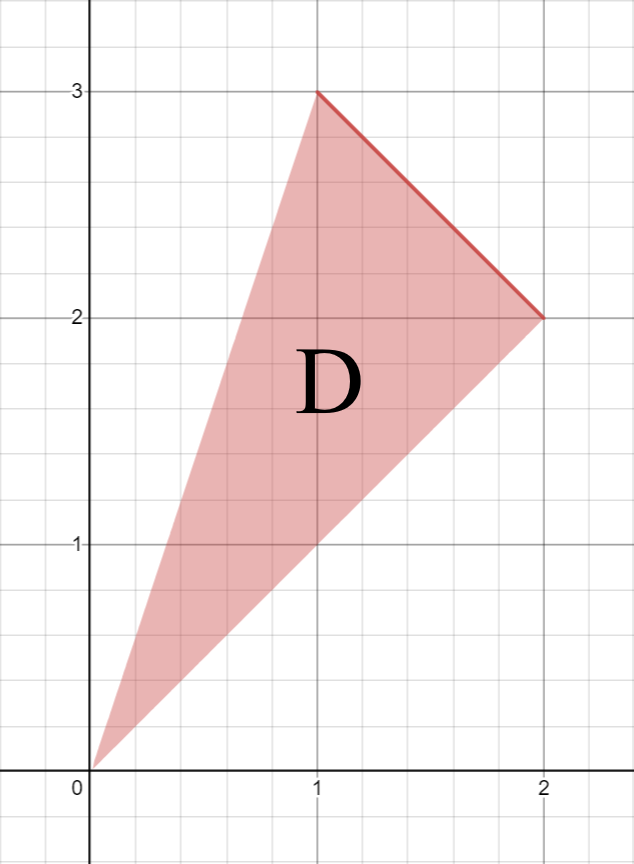
\includegraphics[height=0.35\textwidth]{Pictures/Tutorial 5-1.png}
        \quad 
        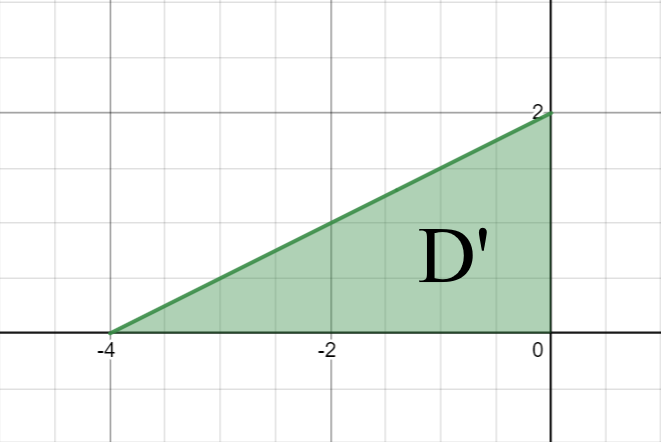
\includegraphics[height=0.35\textwidth]{Pictures/Tutorial 5-2.png}
        \caption{Domains of integration \(D\) in the \(xy\) plane and \(D'\) in the \(uv\) plane.}
    \end{figure}
    
    These functions were chosen such that the point \((x, y) = (1, 3)\) is mapped to the \(v\)-axis and the point \((x, y) = (2, 2)\) is mapped to the \(u\)-axis.
    
    Other change of variables may also be correct.
    
    By observation, we find that the bounds of our integral in terms of \(u\) and \(v\) should be:
    \begin{align}
        -4 \leq & \ u \leq 0 & 0 \leq & \ v \leq \frac{u}{2} + 2
    \end{align}
    
    We now compute the absolute value of the Jacobian:
    \begin{align*}
        \left|\frac{\partial(x, y)}{\partial(u, v)}\right| &= \left|\frac{\partial(u, v)}{\partial(x, y) }\right|^{-1} \\
        &= \left|\begin{vmatrix}
            \frac{\partial u}{\partial x} & \frac{\partial u}{\partial y} \\
            \frac{\partial v}{\partial x} & \frac{\partial v}{\partial y}
        \end{vmatrix}\right|^{-1} \\
        &= \left|\begin{vmatrix}
            -3 & 1 \\
            -1 & 1
        \end{vmatrix}\right|^{-1} \\
        &= \left|-3 + 1\right|^{-1} \\
        &= 2^{-1} \\
        &= \frac{1}{2}
    \end{align*}
    
    By Fubini's Theorem, we may switch our order of integration (this is not necessary, but can be useful): \(dudv \rightarrow dvdu\)
    \begin{align*}
        \iint_D e^{x - y} \ dxdy &= \iint_{D'} e^{-v} \left|\frac{\partial(x, y)}{\partial(u, v) }\right| \ dudv \\
        &= \iint_{D'} e^{-v} \left|\frac{\partial(x, y)}{\partial(u, v) }\right| \ dvdu \\
        &= \frac{1}{2} \int_{-4}^{0} \int_{0}^{\frac{u}{2}+2} e^{-v} \ dvdu \\
        &= \frac{1}{2} \int_{-4}^{0} -e^{-v} \Big|_{0}^{\frac{u}{2}+2} \ du \\
        &= \frac{1}{2} \int_{-4}^{0} -e^{-\frac{u}{2} - 2} + e^0 \ du \\
        &= -\frac{1}{2} \int_{-4}^{0} e^{-\frac{u}{2} - 2} - 1 \ du \\
        &= -\frac{1}{2} \int_{-4}^{0} e^{-\frac{u}{2} - 2} - 1 \ du \\
        &= -\frac{1}{2} \left( -2e^{-\frac{u}{2} - 2} - u\right)\Big|_{-4}^{0} \\
        &= -\frac{1}{2} \left( -2e^{- 2} + 2e^{2 - 2} - 0 -4\right) \\
        &= -\frac{1}{2} \left( -2e^{- 2} + 2 -4\right) \\
        &= -\frac{1}{2} \left( -2e^{- 2} - 2\right) \\
        &= e^{-2} + 1
    \end{align*}
\end{solution}

\newpage 

\begin{solution}
    \textit{(Splitting the domain of integration)}
    
    \begin{figure}[h!]
        \centering
        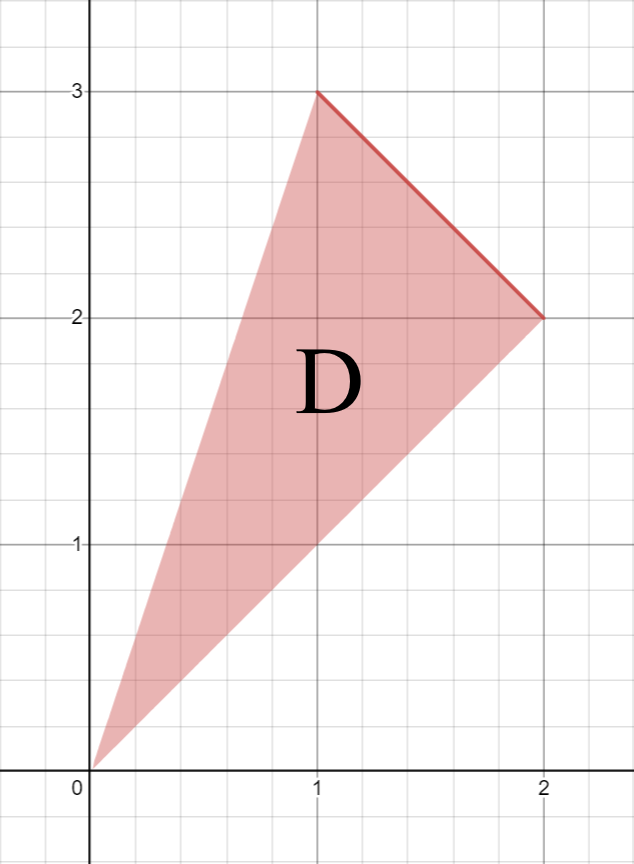
\includegraphics[width=0.3\textwidth]{Pictures/Tutorial 5-1.png} \quad
        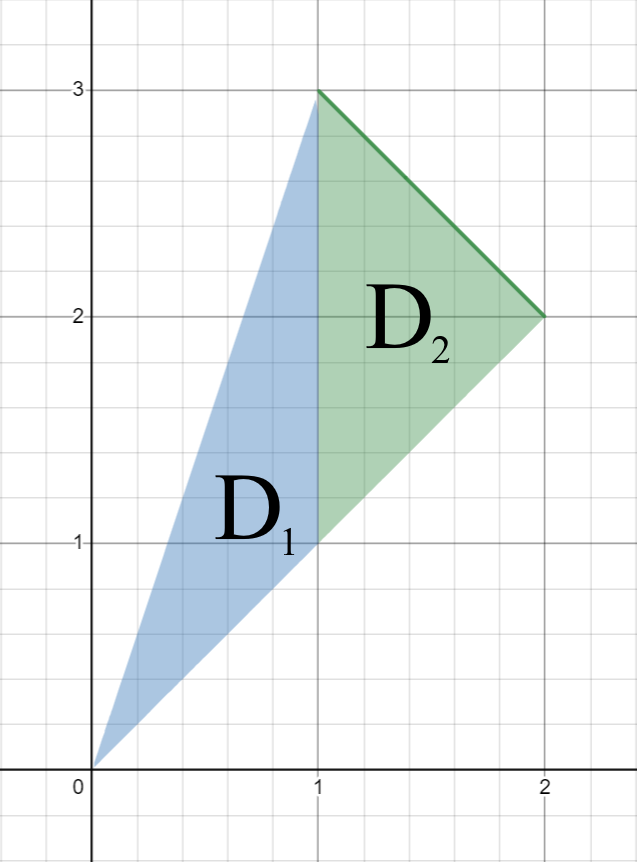
\includegraphics[width=0.3\textwidth]{Pictures/Tutorial 5-3.png} \quad 
        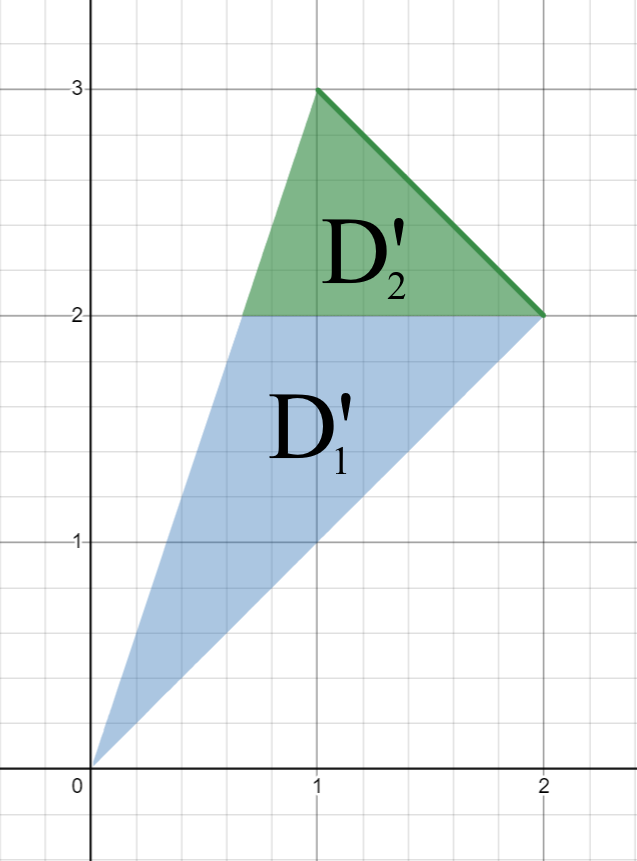
\includegraphics[width=0.3\textwidth]{Pictures/Tutorial 5-4.png}
        \caption{Splitting the domain of integration \(D\) into \(D_1\) and \(D_2\) and/or \(D_1'\) and \(D_2'\).}
    \end{figure}
    
    By Fubini's Theorem, we may switch our order of integration: \(dxdy \rightarrow dydx\)
    \begin{align*}
        \iint_D e^{x-y} \ dxdy &= \iint_{D_1} e^{x-y} \ dxdy + \iint_{D_2} e^{x-y} \ dxdy \\
        &= \int_0^1 \int_x^{3x} e^{x-y} \ dydx + \int_1^2 \int_x^{4 - x} e^{x-y} \ dydx \\
        &= - \int_0^1 e^{x-y} \Big|_x^{3x} \ dx - \int_1^2 e^{x-y}\Big|_x^{4 - x} \ dx \\
        &= - \int_0^1 e^{x-3x} - e^{x-x} \ dx - \int_1^2 e^{x- 4 + x} - e^{x-x} \ dx \\
        &= - \int_0^1 e^{-2x} - 1 \ dx - \int_1^2 e^{2x - 4} - 1 \ dx \\
        &= \frac{e^{-2x}}{2}\Biggr|_0^1 + x\Big|_0^1 - \frac{e^{2x - 4}}{2}\Biggr|_1^2 + x\Big|_1^2 \\
        &= \frac{e^{-2}}{2} - \frac{e^0}{2} + 1 - \frac{e^{4 - 4}}{2} + \frac{e^{2 - 4}}{2} + 2 - 1 \\
        &= \frac{e^{-2}}{2} - \frac{1}{2} + 1 - \frac{1}{2} + \frac{e^{-2}}{2} + 1 \\
        &= e^{-2} + 1
    \end{align*}
    
    We may also evaluate the integral without switching the order of integration (but you'll have \(x\) as a function of \(y\) and no one likes that):
    \begin{align*}
        \iint_D e^{x-y} \ dxdy &= \iint_{D'_1} e^{x-y} \ dxdy + \iint_{D'_2} e^{x-y} \ dxdy \\
        &= \int_0^2 \int_{\frac{y}{3}}^{y} e^{x-y} \ dxdy + \int_2^3 \int_{\frac{y}{3}}^{4 - y} e^{x-y} \ dxdy \\
        &= ... \\
        &= e^{-2} + 1
    \end{align*}
\end{solution}

\subsection{Section 5.5}

\begin{tcolorbox}[
        title={Problem 30 (a)},
        valign=center,
        nobeforeafter,
        colframe=gray!95!black
    ]
    
    Let \(W\) be the region bounded by the planes \(x = 0\), \(y = 0\), \(z = 0\), \(x + y = 1\), and \(x + y = z\). \\
    
    Find the volume of \(W\) and evaluate:
    \begin{align}
        &\iiint_W x \ dxdydz & &\iiint_W y \ dxdydz
    \end{align}
\end{tcolorbox}

\begin{solution}
    Recall that the volume of region \(W\) is given by:
    \begin{align}
        V(W) &= \iiint_W dxdydz
    \end{align}
    
    \begin{figure}[h!]
        \centering
        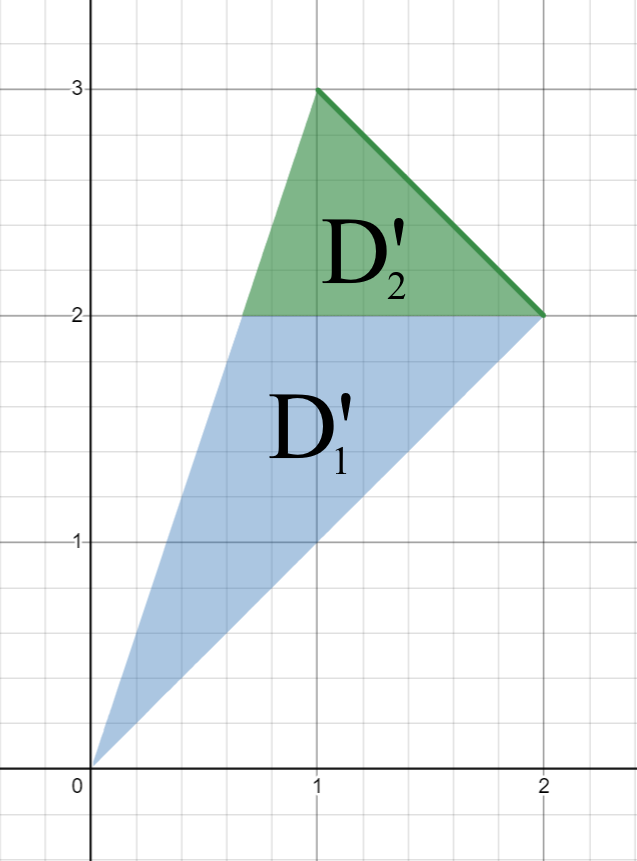
\includegraphics[width=0.47\textwidth]{Pictures/Tutorial 5-4.png} \\
        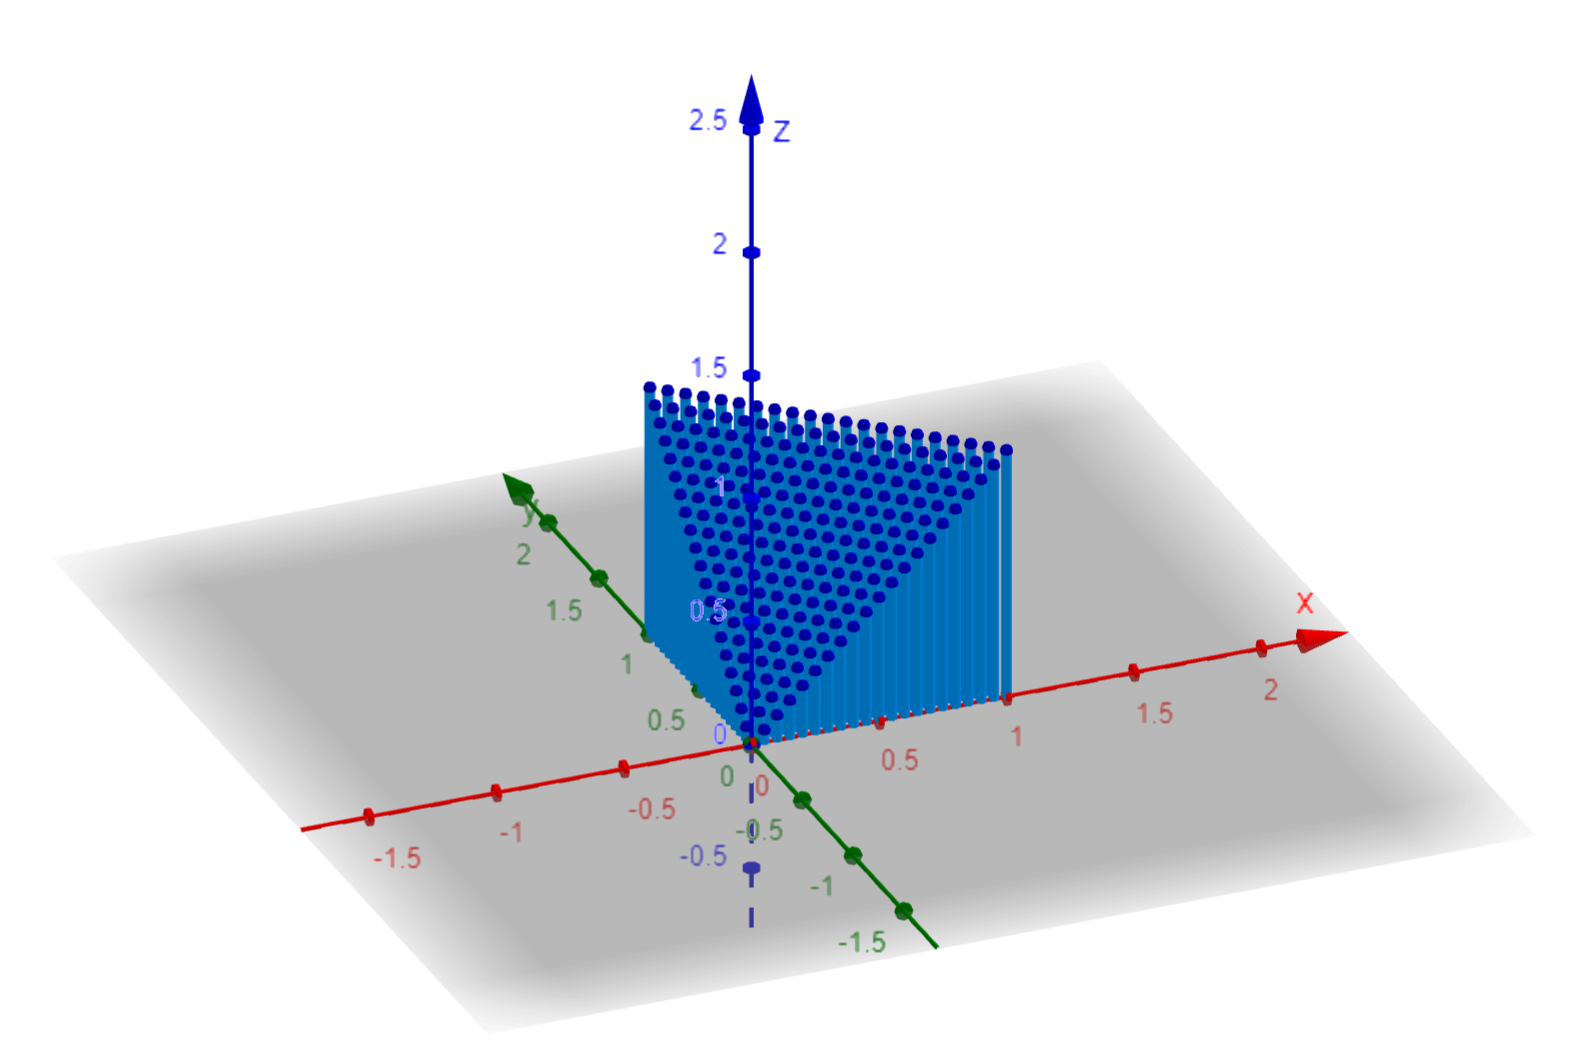
\includegraphics[width=0.47\textwidth]{Pictures/Tutorial 5-5.png} 
        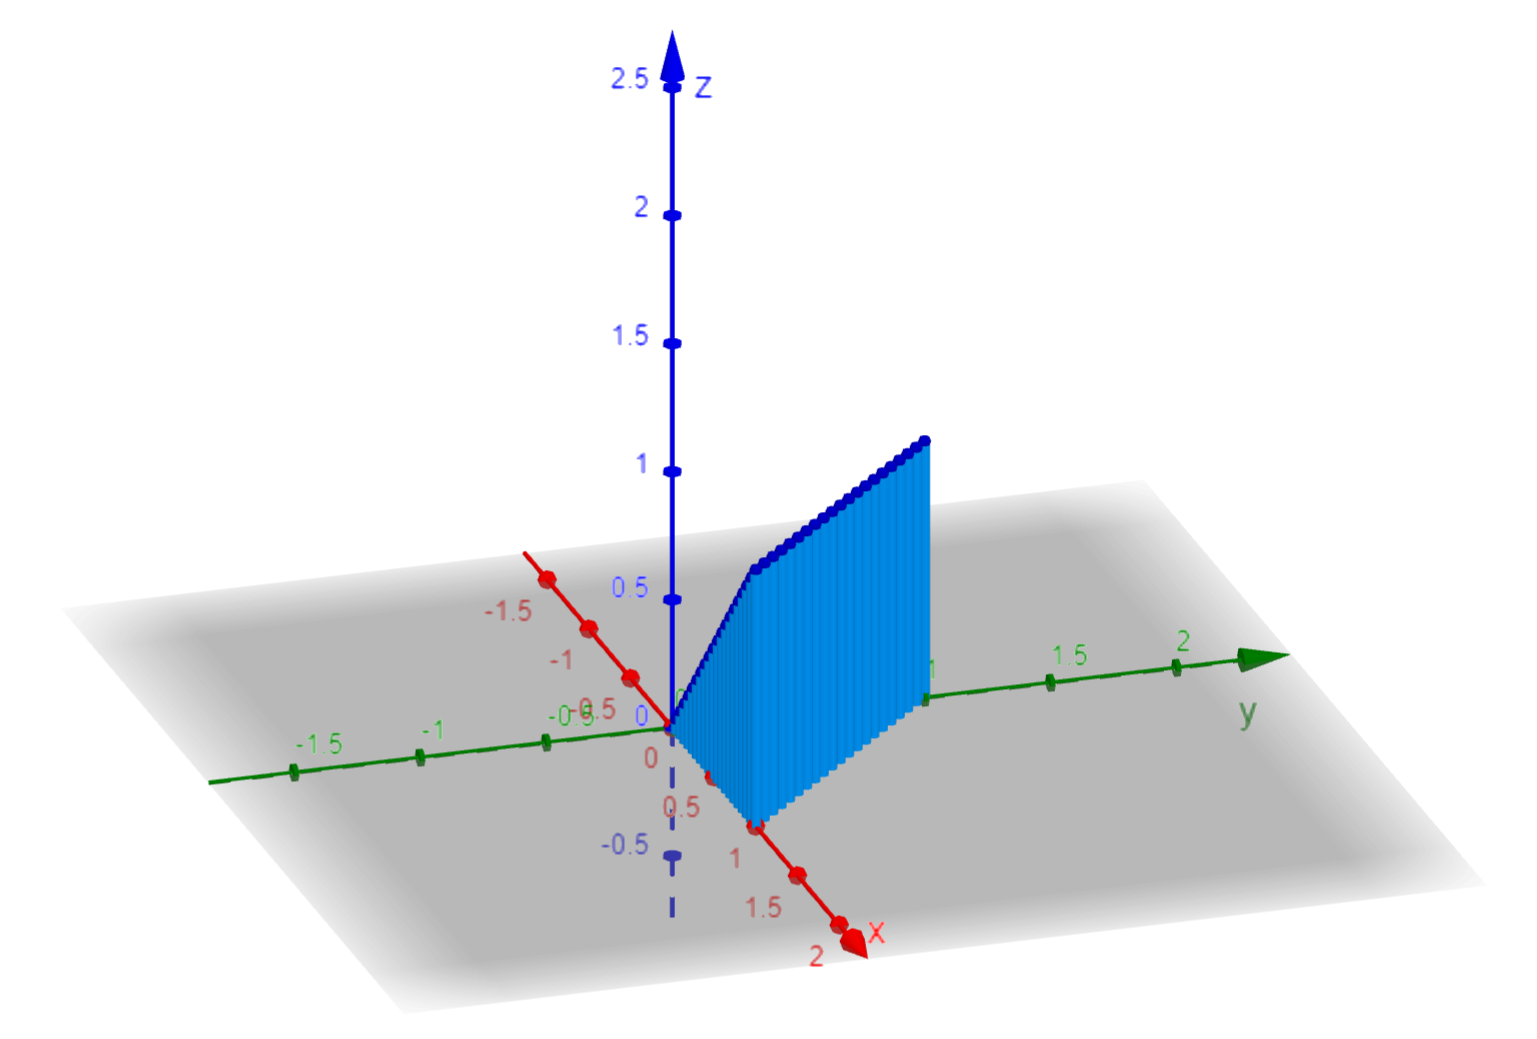
\includegraphics[width=0.47\textwidth]{Pictures/Tutorial 5-6.png}
        \caption{Visualizing the region \(W\) in 3D.}
    \end{figure}
    
    By observation, the lower bounds of \(x\), \(y\), and \(z\) are equal to zero.
    
    The upper bound of \(z\) is given to be \(z = x + y\).
    
    The upper bound of \(y\) is found to be \(y = 1 - x\). 
    
    The upper bound of \(x\) is found to be \(x = 1\).
    
    The bounds of our integral should therefore be:
    \begin{align}
        0 \leq & \ z \leq x + y & 0 \leq & \ y \leq 1 - x & 0 \leq & \ x \leq 1
    \end{align}
    
    By Fubini's Theorem, we may switch our order of integration: \(dxdydz \rightarrow dzdydx\)
    \begin{align*}
        \iiint_W dxdydz &= \int_0^1 \int_0^{1 - x}\int_0^{x + y} dzdydx \\
        &= \int_0^1 \int_0^{1 - x} z \Big|_{0}^{x + y} \ dydx \\
        &= \int_0^1 \int_0^{1 - x}x + y \ dydx \\
        &= \int_0^1 \left(xy + \frac{y^2}{2}\right) \Big|_0^{1 - x} \ dx \\
        &= \int_0^1 x(1 - x) + \frac{(1 - x)^2}{2} \ dx \\
        &= \int_0^1 x - x^2 + \frac{(1 - x)^2}{2} \ dx \\
        &= \left(\frac{x^2}{2} - \frac{x^3}{3} - \frac{(1 - x)^3}{6}\right) \Biggr|_0^1 \\
        &= \frac{1}{2} - \frac{1}{3} + \frac{1}{6} \\
        &= \frac{1}{3}
    \end{align*}
    
    We now evaluate the other two integrals:
    \begin{align*}
        \iiint_W x \ dxdydz &= \int_0^1 \int_0^{1 - x}\int_0^{x + y} x \ dzdydx \quad \quad \quad \quad \quad \quad & \iiint_W y \ dxdydz &= \int_0^1 \int_0^{1 - x}\int_0^{x + y} y \ dzdydx \\
        &= \int_0^1 \int_0^{1 - x} xz \Big|_{0}^{x + y} \ dydx & &= \int_0^1 \int_0^{1 - x} yz \Big|_{0}^{x + y} \ dydx \\
        &= \int_0^1 \int_0^{1 - x} x(x + y) \ dydx & &= \int_0^1 \int_0^{1 - x} y(x + y) \ dydx \\
        &= \int_0^1 \int_0^{1 - x} x^2 + xy \ dydx & &= \int_0^1 \int_0^{1 - x} xy + y^2 \ dydx \\
        &= \int_0^1 \left(x^2y + \frac{xy^2}{2}\right) \Biggr|_0^{1 - x} \ dx & &= \int_0^1 \left(\frac{xy^2}{2} + \frac{y^3}{3}\right)\Biggr|_0^{1 - x} \ dx \\
        &= \int_0^1 x^2(1 - x) + \frac{x(1 - x)^2}{2} \ dx & &= \int_0^1 \frac{x(1 - x)^2}{2} + \frac{(1 - x)^3}{3} \ dx \\
        &= -\frac{x^4 - 2x^2}{8} \Biggr|_0^1 & &= -\frac{x^4 - 2x^2}{8} \Biggr|_0^1 \\
        &= -\frac{1 - 2}{8} & &= -\frac{1 - 2}{8} \\
        &= \frac{1}{8} & &= \frac{1}{8} 
    \end{align*}
\end{solution}

\newpage 

\setcounter{section}{6}
\section{\centering Tutorial 6}

\subsection{Section 6.2}

\begin{tcolorbox}[
        title={Problem 10},
        valign=center,
        nobeforeafter,
        colframe=gray!95!black
    ]
    
    Calculate:
    \begin{align}
        \iint_R \frac{1}{x + y} \ dydx
    \end{align}
    
    where \(R\) is the region bounded by \(x = 0\), \(y = 0\), \(x + y = 1\), \(x + y = 4\), by using the mapping \(T(u, v) = (u - uv, uv)\).
\end{tcolorbox}

\begin{solution}
     We first find the bounds of our integral in terms of \(u\) and \(v\). 
    
    We require that:
    \begin{align*}
        x + y &\geq 1 & x + y &\leq 4 \\
        u - uv + uv &\geq 1 & u - uv + uv &\leq 4 \\
        u &\geq 1 & u &\leq 4
    \end{align*}
    This implies that \(1 \leq u \leq 4\).
    
    We also require that:
    \begin{align*}
        x &\geq 0 & y &\geq 0 \\
        u - uv &\geq 0 & uv &\geq 0 \\
        u &\geq uv & v &\geq 0 \\
        1 &\geq v
    \end{align*}
    This implies that \(0 \leq v \leq 1\).
    
    We now compute the absolute value of the Jacobian:
    \begin{align*}
        \left|\frac{\partial(x, y)}{\partial(u, v)}\right| &= \left|\begin{vmatrix}
            \frac{\partial x}{\partial u} & \frac{\partial x}{\partial v} \\
            \frac{\partial y}{\partial u} & \frac{\partial y}{\partial v}
        \end{vmatrix}\right| \\
        &= \left|\begin{vmatrix}
            1 - v & -u \\
            v & u
        \end{vmatrix}\right| \\
        &= \left|(1-v)u + uv\right| \\
        &= \left|u - uv + uv\right| \\
        &= |u| \\
        &= u
    \end{align*}
    where \(|u| = u\) since \(1 \leq u \leq 4\). 
    
   Then the integral in the new coordinate system is given by:
    \begin{align*}
        \iint_R \frac{1}{x + y} \ dydx &= \iint_{R'} \frac{1}{u - uv + uv} \left|\frac{\partial(x, y)}{\partial(u, v)}\right| \ du dv \\
        &= \int_{0}^{1} \int_{1}^4 \frac{u}{u} \ du dv \\
        &= \int_{0}^{1} (4 - 1) \ dv \\
        &= 3 \int_{0}^{1} dv \\
        &= 3
    \end{align*}
\end{solution}

\begin{tcolorbox}[
        title={Problem 36 (a)},
        valign=center,
        nobeforeafter,
        colframe=gray!95!black
    ]
    Let \(R\) denote the region inside \(x^2 + y^2 = 1\), but outside \(x^2 + y^2 = 2y\) with \(x \geq 0\) and \(y \geq 0\). \\
    
    Sketch this region.
\end{tcolorbox}

\begin{solution}
    The region inside \(x^2 + y^2 = 1\) with \(x \geq 0\) and \(y \geq 0\) is given by:
    \begin{figure}[h!]
        \centering
        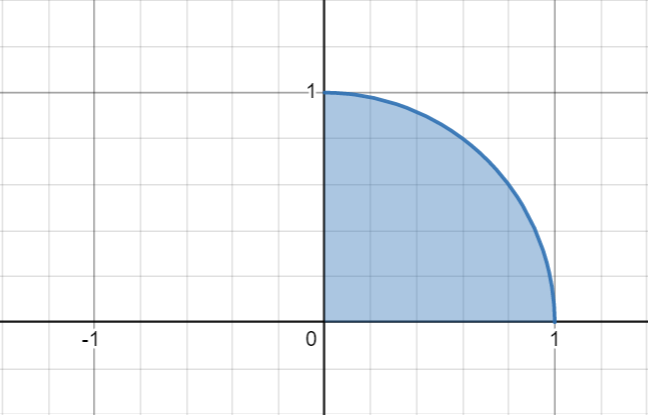
\includegraphics[width=0.6\textwidth]{Pictures/Tutorial 6-1.png}
        \caption{Unit disk centered at the origin, restricted to the first quadrant of the coordinate plane.}
    \end{figure}
    
    The region outside \(x^2 + y^2 = 2y\) requires some manipulation. 
    
    Observe:
    \begin{align*}
        x^2 + y^2 &= 2y \\
        x^2 + y^2 - 2y &= 0 \\
        x^2 + y^2 - 2y + 1 &= 1 \\
        x^2 + (y - 1)^2 &= 1
    \end{align*}
    
    By completing the square, we can see that this constraint takes the form of a unit disk centered at \((x, y) = (0, 1)\). 
    
    The region outside \(x^2 + y^2 = 2y\) with \(x \geq 0\) and \(y \geq 0\) is given by:
    \begin{figure}[h!]
        \centering
        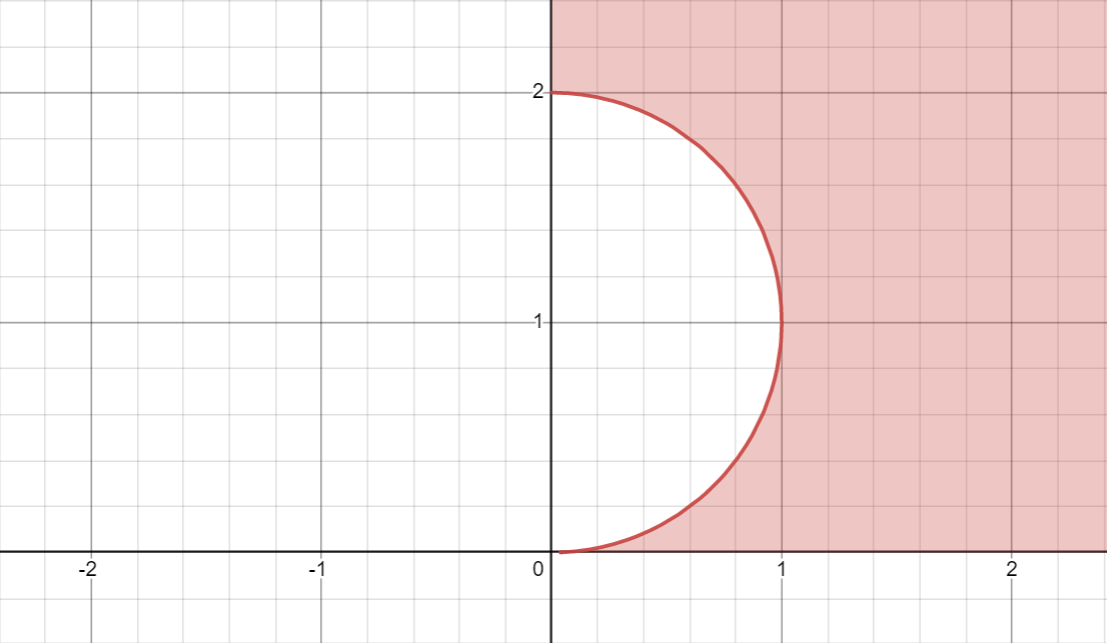
\includegraphics[width=0.6\textwidth]{Pictures/Tutorial 6-2.png}
        \caption{Unit disk centered at the point \((x, y) = (0, 1)\), restricted to the first quadrant of the coordinate plane.}
    \end{figure}
    
    \newpage
    Combined, we obtain the following region:
    \begin{figure}[h!]
        \centering
        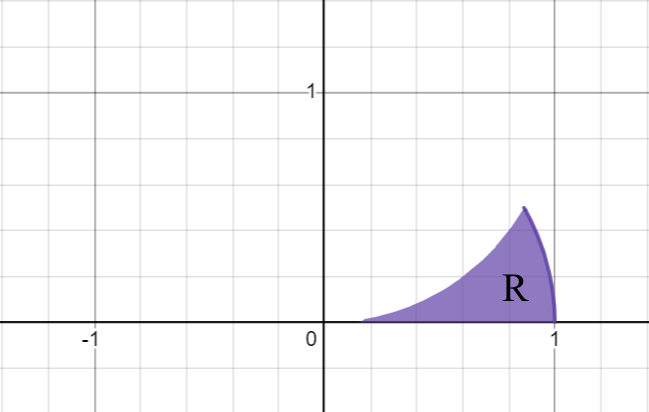
\includegraphics[width=0.6\textwidth]{Pictures/Tutorial 6-3.png}
        \caption{Intersection of the two previous regions.}
    \end{figure}
\end{solution}

\begin{tcolorbox}[
        title={Problem 36 (b)},
        valign=center,
        nobeforeafter,
        colframe=gray!95!black
    ]
    Let \(u = x^2 + y^2\) and \(v = x^2 + y^2 - 2y\). \\
    
    Sketch the region \(R'\) in the \(uv\) plane which corresponds to \(R\) under this change of coordinates.
\end{tcolorbox}

\begin{solution}
    We first isolate for \(y\):
    \begin{align*}
        v &= x^2 + y^2 - 2y \\
        v &= u - 2y \\
        y &= \frac{u - v}{2}
    \end{align*}
    
    We require that:
    \begin{align*}
        x^2 + y^2 &\leq 1 & x^2 + y^2 &\geq 2y\\
        u &\leq 1 & u &\geq u - v \\
        & & 0 &\geq - v \\
        & & v &\geq 0
    \end{align*}
    since \(x^2 + y^2 \geq 0\) always, it follows that \(0 \leq u \leq 1\).
    
    To find the upper bound for \(v\), we also require that \(y \geq 0\):
    \begin{align*}
        y &\geq 0 \\
        \frac{u - v}{2} &\geq 0 \\
        u &\geq v
    \end{align*}
    
    The bounds of our integral in terms of \(u\) and \(v\) should therefore be:
    \begin{align}
        0 \leq &u \leq 1 & 0 \leq v \leq u 
    \end{align}
    
    \begin{figure}[h!]
        \centering
        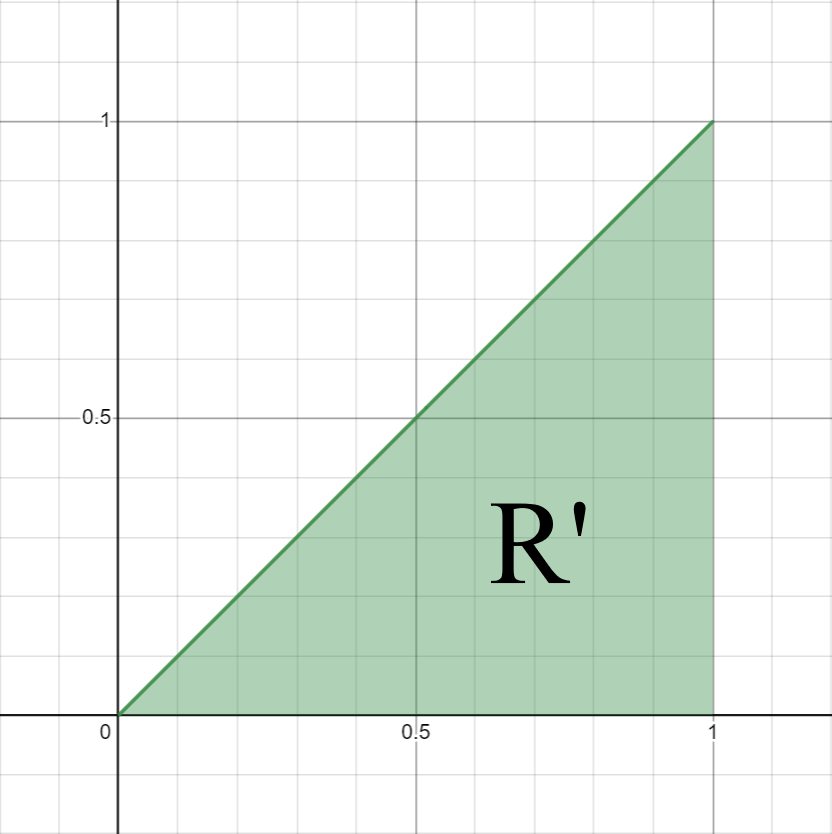
\includegraphics[width=0.4\textwidth]{Pictures/Tutorial 6-4.png}
        \caption{Domain of integration \(R'\) in the \(uv\) plane.}
    \end{figure}
\end{solution}

\begin{tcolorbox}[
        title={Problem 36 (c)},
        valign=center,
        nobeforeafter,
        colframe=gray!95!black
    ]
    Compute:
    \begin{align}
        \iint_R xe^y \ dxdy
    \end{align}
    using the previously mentioned change of coordinates.
\end{tcolorbox}

\begin{solution}
    We first compute the Jacobian:
    \begin{align*}
        \left|\frac{\partial(x, y)}{\partial(u, v)}\right| &= \left|\frac{\partial(u, v)}{\partial(x, y)}\right|^{-1} \\
        &= \left|\begin{vmatrix}
            \frac{\partial u}{\partial x} & \frac{\partial u}{\partial y} \\
            \frac{\partial v}{\partial x} & \frac{\partial v}{\partial y}
        \end{vmatrix}\right|^{-1} \\
        &= \left|\begin{vmatrix}
            2x & 2y \\
            2x & 2y - 2
        \end{vmatrix}\right|^{-1} \\
        &= \left|2x(2y - 2) - 2x(2y)\right|^{-1} \\
        &= \left|4xy - 4x - 4xy\right|^{-1} \\
        &= \left|-4x\right|^{-1} \\
        &= \frac{1}{4|x|} \\
        &= \frac{1}{4x}
    \end{align*}
    where \(|x| = x\) since \(x \geq 0\).
    
    Then the integral in the new coordinate system is given by:
    \begin{align*}
        \iint_R xe^y \ dxdy &= \iint_{R'} xe^{\frac{u - v}{2}} \left|\frac{\partial(x, y)}{\partial(u, v)}\right| \ du dv \\
        &= \frac{1}{4} \int_{0}^{1} \int_{0}^{u} \frac{x}{x}e^{\frac{u - v}{2}} \ du dv \\
        &= \frac{1}{4} \int_{0}^{1} \int_{0}^{u} e^{\frac{u - v}{2}} \ dv du \\
        &= \frac{1}{4} \int_{0}^{1} -2 e^{\frac{u - v}{2}} \Big|_{0}^{u} \ du \\
        &= \frac{1}{4} \int_{0}^{1} -2 e^{0} + 2 e^{\frac{u}{2}} \ du \\
        &= \frac{1}{2} \int_{0}^{1} e^{\frac{u}{2}} - 1 \ du \\
        &= \frac{1}{2} \left( 2 e^{\frac{u}{2}} - u\right)\Big|_{0}^{1} \\
        &= \frac{1}{2} \left( 2 e^{\frac{1}{2}} - 2e^0 - 1\right) \\
        &= \frac{1}{2} \left( 2 e^{\frac{1}{2}} - 3\right) \\
        &= e^{\frac{1}{2}} - \frac{3}{2}
    \end{align*}
\end{solution}

\newpage 

\setcounter{section}{7}
\section{\centering Tutorial 7}

\subsection{Section 7.3}

\begin{tcolorbox}[
        title={Problem 16},
        valign=center,
        nobeforeafter,
        colframe=gray!95!black
    ]
    Find a parametrization of the surface
    \begin{align}
        x^3 + 3xy + z^2 &= 2
    \end{align}
    where \(z \geq 0\). \\
    
    Use it to find the tangent plane at the point \((x, y, z) = \left(1, \frac{1}{3}, 0\right)\).
\end{tcolorbox}

\begin{solution}
    Recall that we parametrize a surface using the function \(\Phi: D \subset \mathbb{R}^2 \rightarrow S \subset \mathbb{R}^3\):
    \begin{align}
        \Phi(u, v) &= (x, y, z)
    \end{align}
    
    Observe that it is easier to isolate for \(y\) in terms of \(x\) and \(z\). This is because there is a cubed term in \(x\) and a squared term in \(z\).
    
    We therefore parametrize this surface by first setting \(x = u\) and \(z = v\).
    
    Isolating for \(y\):
    \begin{align*}
        2 &= x^3 + 3xy + z^2 \\
        -3xy &= x^3 + z^2 - 2 \\
        y &= -\frac{x^3 + z^2 - 2}{3x} \\
        y &= -\frac{x^2}{3} - \frac{z^2}{3x} + \frac{2}{3x} \\
        y &= -\frac{u^2}{3} - \frac{v^2}{3u} + \frac{2}{3u}
    \end{align*}
    
    Then:
    \begin{align}
        \Phi(u, v) &= \left(u, -\frac{u^2}{3} - \frac{v^2}{3u} + \frac{2}{3u}, v\right)
    \end{align}
    
    In order to find the tangent plane at a given point, we must first compute the normal vector of the surface at that point.
    
    Recall that the normal vector of the parametrized surface is given by:
    \begin{align}
        \vec{n} &= \Phi_u \times \Phi_v
    \end{align}
    
    We now compute the partial derivatives of \(\Phi\):
    \begin{align}
        \Phi_u &= \left(1, -\frac{2u}{3} + \frac{v^2}{3u^2} - \frac{2}{3u^2}, 0\right) & \Phi_v &= \left(0, - \frac{2v}{3u}, 1\right)
    \end{align}
    
    Observe that the point \((x, y, z) = \left(1, \frac{1}{3}, 0\right)\) is given by \((u, v) = (1, 0)\).
    
    Then the normal at the point \((x, y, z) = \left(1, \frac{1}{3}, 0\right)\) is given by:
    \begin{align*}
        \vec{n} &= \Phi_u(1, 0) \times \Phi_v(1, 0) \\
        &= \left(1, -\frac{2(1)}{3} + \frac{(0)^2}{3(1)^2} - \frac{2}{3(1)^2}, 0\right) \times \left(0, - \frac{2(0)}{3(1)}, 1\right) \\
        &= \left(1, -\frac{2}{3} - \frac{2}{3}, 0\right) \times \left(0, 0, 1\right) \\
        &= \left(1, -\frac{4}{3}, 0\right) \times \left(0, 0, 1\right) \\
        &= \left(1, -\frac{4}{3}, 0\right) \times \left(0, 0, 1\right) \\
        &= \left(-\frac{4}{3}, -1, 0\right)
    \end{align*}
    
    Recall that the equation of the plane tangent to the point \((x_0, y_0, z_0)\) is given by:
    \begin{align}
        \vec{n} \cdot \left((x, y, z) - (x_0, y_0, z_0)\right) &= 0 \\
        \vec{n} \cdot \left(x - x_0, y - y_0, z - z_0\right) &= 0
    \end{align}
    
    Then the equation of the plane tangent to the point \(\left(1, \frac{1}{3}, 0\right)\) is given by:
    \begin{align*}
        \vec{n} \cdot \left(x - x_0, y - y_0, z - z_0\right) &= 0 \\
        \left(-\frac{4}{3}, -1, 0\right) \cdot \left(x - 1, y - \frac{1}{3}, z\right) &= 0 \\
        -\frac{4}{3}(x - 1) - \left(y - \frac{1}{3}\right) &= 0 \\
        -\frac{4}{3}x + \frac{4}{3} - y + \frac{1}{3} &= 0 \\
        \frac{4}{3}x + y - \frac{5}{3} &= 0
    \end{align*}
    
\end{solution}

\begin{tcolorbox}[
        title={Problem 18},
        valign=center,
        nobeforeafter,
        colframe=gray!95!black
    ]
    Given a sphere of radius 2 centered at the origin, find the equation for the plane tangent to it at the point \((1, 1, \sqrt{2})\) by considering the sphere as:
    
    \begin{itemize}
        \item a sphere parametrized by \(\Phi(\theta, \phi) = (2\cos(\theta)\sin(\phi), 2\sin(\theta)\sin(\phi), 2\cos(\phi))\)
        \item a level surface of \(f(x, y, z) = x^2 + y^2 + z^2\)
        \item the graph of \(g(x, y) = \sqrt{4 - x^2 - y^2}\)
    \end{itemize}
\end{tcolorbox}

\begin{solution}
\textit{(Parametrization)}

Recall that for an arbitrary parametrization \(\Phi(u, v)\), the vector \(\Phi_u \times \Phi_v\) is the normal vector to the parametrized surface \(S\).

Then the vector \(\Phi_\theta \times \Phi_\phi\) is the normal vector of the sphere.

We compute the partial derivatives of \(\Phi\):
\begin{align*}
    \Phi_\theta &= (-2\sin(\theta)\sin(\phi), 2\cos(\theta)\sin(\phi), 0) & \Phi_\phi &= (2\cos(\theta)\cos(\phi), 2\sin(\theta)\cos(\phi), -2\sin(\phi))
\end{align*}

Observe that the point \((1, 1 \sqrt{2})\) is given by \((\theta, \phi) = \left(\frac{\pi}{4}, \frac{\pi}{4}\right)\). 

This can be found by equating the point of interest with the parametrization and solving for \(\theta\) and \(\phi\) component-wise:
\begin{align*}
    (1, 1 \sqrt{2}) &= (2\cos(\theta)\sin(\phi), 2\sin(\theta)\sin(\phi), 2\cos(\phi))
\end{align*}

We first solve for \(\phi\) by analyzing the \(z\) component:
\begin{align*}
    2\cos{\phi} &= \sqrt{2} \\
    \cos{\phi} &= \frac{\sqrt{2}}{2} \\
    \phi &= \pm \frac{\pi}{4}
\end{align*}

By convention, \(\phi \in [0, \pi]\). Therefore, \(\phi = \frac{\pi}{4}\).

We now solve for \(\theta\) by analyzing the \(x\) and \(y\) components:
\begin{align*}
    2\cos(\theta)\sin(\phi) &= 1 & 2\sin(\theta)\sin(\phi) &= 1 \\
    2\cos(\theta)\sin\left(\frac{\pi}{4}\right) &= 1 & 2\sin(\theta)\sin\left(\frac{\pi}{4}\right) &= 1 \\
    2\cos(\theta)\frac{\sqrt{2}}{2} &= 1 & 2\sin(\theta)\frac{\sqrt{2}}{2} &= 1 \\
    \sqrt{2} \cos(\theta) &= 1 & \sqrt{2} \sin(\theta) &= 1 \\
    \cos(\theta) &= \frac{1}{\sqrt{2}} & \sin(\theta) &= \frac{1}{\sqrt{2}} \\
    \theta &= \pm \frac{\pi}{4} & \theta &= \frac{\pi}{4} \text{ or } \frac{3\pi}{4}
\end{align*}

Both conditions hold when \(\theta = \frac{\pi}{4}\).

Then the normal at the point \((1, 1 \sqrt{2})\) is given by:
\begin{align*}
    \vec{n} &= \Phi_\theta\left(\frac{\pi}{4}, \frac{\pi}{4}\right) \times \Phi\left(\frac{\pi}{4}, \frac{\pi}{4}\right) \\
    &= \left(-2\sin\left(\frac{\pi}{4}\right)\sin\left(\frac{\pi}{4}\right), 2\cos\left(\frac{\pi}{4}\right)\sin\left(\frac{\pi}{4}\right), 0\right) \times \left(2\cos\left(\frac{\pi}{4}\right)\cos\left(\frac{\pi}{4}\right), 2\sin\left(\frac{\pi}{4}\right)\cos\left(\frac{\pi}{4}\right), -2\sin\left(\frac{\pi}{4}\right)\right) \\
    &= \left(-2\frac{\sqrt{2}}{2}\frac{\sqrt{2}}{2}, 2\frac{\sqrt{2}}{2}\frac{\sqrt{2}}{2}, 0\right) \times \left(2\frac{\sqrt{2}}{2}\frac{\sqrt{2}}{2}, 2\frac{\sqrt{2}}{2}\frac{\sqrt{2}}{2}, -2\frac{\sqrt{2}}{2}\right) \\
    &= \left(-\frac{2}{2}, \frac{2}{2}, 0\right) \times \left(\frac{2}{2}, \frac{2}{2}, -\sqrt{2}\right) \\
    &= \left(-1, 1, 0\right) \times \left(1, 1, -\sqrt{2}\right) \\
    &= \left(\sqrt{2}, \sqrt{2}, 2\right)
\end{align*}

Recall that the equation of the plane tangent to the point \((x_0, y_0, z_0)\) is given by:
    \begin{align}
        \vec{n} \cdot \left((x, y, z) - (x_0, y_0, z_0)\right) &= 0 \\
        \vec{n} \cdot \left(x - x_0, y - y_0, z - z_0\right) &= 0
    \end{align}
    
    Then the equation of the plane tangent to the point \(\left(1, 1, \sqrt{2}\right)\) is given by:
    \begin{align*}
        \vec{n} \cdot \left(x - x_0, y - y_0, z - z_0\right) &= 0 \\
        \left(\sqrt{2}, \sqrt{2}, 2\right) \cdot \left(x - 1, y - 1, z - \sqrt{2}\right) &= 0 \\
        \sqrt{2}(x - 1) + \sqrt{2}(y - 1) + 2\left(z - \sqrt{2}\right) &= 0 \\
        \sqrt{2}x - \sqrt{2} + \sqrt{2}y - \sqrt{2} + 2z - 2\sqrt{2} &= 0 \\
        \sqrt{2}x + \sqrt{2}y + 2z - 4\sqrt{2} &= 0 \\
        x + y + \sqrt{2}z - 4 &= 0
    \end{align*}

\end{solution}

\begin{solution}
\textit{(Level surface)}
    
    Observe that the sphere of radius 2 centered at the origin is equal to the level surface of \(f\) where \(f(x, y, z) = 4\).
    
    Recall that the gradient of \(f\) is perpendicular to every level surface of \(f\). The normal vector is therefore parallel to the gradient of \(f\).
    
    We first compute the gradient of \(f\):
    \begin{align}
        \nabla f &= (2x, 2y, 2z)
    \end{align}
    
    Then the normal at the point \((x, y, z) = (1, 1, \sqrt{2})\) is given by:
    \begin{align*}
        \vec{n} &= \nabla f(1, 1, \sqrt{2}) \\
        &= (2(1), 2(1), 2\sqrt{2}) \\
        &= (2, 2, 2\sqrt{2})
    \end{align*}
    
    Recall that the equation of the plane tangent to the point \((x_0, y_0, z_0)\) is given by:
    \begin{align}
        \vec{n} \cdot \left((x, y, z) - (x_0, y_0, z_0)\right) &= 0 \\
        \vec{n} \cdot \left(x - x_0, y - y_0, z - z_0\right) &= 0
    \end{align}
    
    Then the equation of the plane tangent to the point \(\left(1, 1, \sqrt{2}\right)\) is given by:
    \begin{align*}
        \vec{n} \cdot \left(x - x_0, y - y_0, z - z_0\right) &= 0 \\
        (2, 2, 2\sqrt{2}) \cdot \left(x - 1, y - 1, z - \sqrt{2}\right) &= 0 \\
        2(x - 1) + 2(y - 1) + 2\sqrt{2}(z - \sqrt{2}) &= 0 \\
        2x - 2 + 2y - 2 + 2\sqrt{2}z - 4 &= 0 \\
        2x + 2y + 2\sqrt{2}z - 8 &= 0 \\
        x + y + \sqrt{2}z - 4 &= 0
    \end{align*}
    
\end{solution}

\begin{solution}
\textit{(Graph)}
    
    Recall that the equation of the plane tangent to the graph of \(g\) at \((x_0, y_0, g(x_0, y_0))\) is given by:
    \begin{align}
        z - g(x_0, y_0) &= \frac{\partial g(x_0, y_0)}{\partial x}(x - x_0) + \frac{\partial g(x_0, y_0)}{\partial y}(y - y_0)
    \end{align}
    
    We first calculate the partial derivatives of \(g\):
    \begin{align*}
        \frac{\partial g}{\partial x} &= -\frac{x}{\sqrt{4 - x^2 - y^2}} & \frac{\partial g}{\partial y} &= -\frac{y}{\sqrt{4 - x^2 - y^2}}
    \end{align*}
    
    The equation of the plane tangent to the graph of \(g\) at \((1, 1, \sqrt{2})\) is then given by:
    \begin{align*}
        z - \sqrt{2} &= -\frac{1}{\sqrt{4 - 1^2 - 1^2}}(x - 1) -\frac{1}{\sqrt{4 - 1^2 - 1^2}}(y - 1) \\
        z - \sqrt{2} &= -\frac{1}{\sqrt{4 - 2}}(x - 1) -\frac{1}{\sqrt{4 - 2}}(y - 1) \\
        z - \sqrt{2} &= -\frac{1}{\sqrt{2}}(x - 1) -\frac{1}{\sqrt{2}}(y - 1) \\
        \sqrt{2} z - 2 &= -(x - 1) -(y - 1) \\
        0 &= x - 1 + y - 1 + \sqrt{2} z - 2 \\
        0 &= x + y + \sqrt{2} z - 4
    \end{align*}
\end{solution}

\subsection{Section 7.4}

\begin{tcolorbox}[
        title={Problem 6},
        valign=center,
        nobeforeafter,
        colframe=gray!95!black
    ]
    Find the area of the surface defined by \(z = xy\) and \(x^2 + y^2 \leq 2\).
\end{tcolorbox}

\begin{solution}
    Observe that this surface is given in the form \(z = g(x, y)\). 
    
    Recall that the area of a graph is given by:
    \begin{align}
        A(S) &= \iint_D \sqrt{1 + \|\nabla g\|^2} \ dA
    \end{align}
    
    We first calculate the gradient:
    \begin{align}
        \nabla g &= \left(\frac{\partial g}{\partial x}, \frac{\partial g}{\partial y}\right) \\
        &= \left(y, x\right)
    \end{align}
    
    We now calculate the norm of the gradient:
    \begin{align}
        \|\nabla g\|^2 &= \|\left(y, x\right)\|^2 \\
        &= y^2 + x^2
    \end{align}
    
    The integral is easier to compute in polar coordinates. Therefore, we will compute the integral in polar coordinates.
    
    Recall that:
    \begin{align}
        x &= r\cos(\theta) & y &= r\sin(\theta) & r &= \sqrt{x^2 + y^2}
    \end{align}
    
    Then the domain of integration is given by:
    \begin{align}
        0 \leq & \ r \leq \sqrt{2} & 0 \leq & \ \theta \leq 2\pi
    \end{align}
    
    Recall also that the infinitesimal area element in polar coordinates is given by:
    \begin{align}
        dA &= r \ dr d\theta
    \end{align}
    
    Then the surface area is given by:
    \begin{align}
        A(S) &= \iint_D \sqrt{1 + \|\nabla g\|^2} \ dA \\
        &= \iint_D \sqrt{1 + y^2 + x^2} \ dA \\
        &= \int_0^{2\pi} \int_0^{\sqrt{2}} \sqrt{1 + r^2} \ r \ dr d\theta \\
        &= \int_0^{2\pi} \frac{1}{3}\left(\sqrt{1 + r^2}\right)^{\frac{3}{2}}\Biggr|_0^{\sqrt{2}} d\theta \\
        &= \frac{1}{3}\int_0^{2\pi} \sqrt{1 + \sqrt{2}^2} - \sqrt{1 + 0^2} \ d\theta \\
        &= \frac{1}{3} \int_0^{2\pi} \sqrt{3} - 1 \ d\theta \\
        &= \frac{2\pi}{3} \left(\sqrt{3} - 1\right)
    \end{align}
\end{solution}

\begin{tcolorbox}[
        title={Problem 10},
        valign=center,
        nobeforeafter,
        colframe=gray!95!black
    ]
    Find the area of the portion of the unit sphere that is cut out by the cone \(z \geq \sqrt{x^2 + y^2}\).
\end{tcolorbox}

\begin{solution}
    The intersection of the sphere and the cone is found by equation the following two equations:
    \begin{align*}
        x^2 + y^2 + z^2 &= 1 & z &= \sqrt{x^2 + y^2}
    \end{align*}
    
    We obtain:
    \begin{align*}
        x^2 + y^2 + z^2 &= 1 \\
        x^2 + y^2 + \left(\sqrt{x^2 + y^2}\right)^2 &= 1 \\
        x^2 + y^2 + x^2 + y^2 &= 1 \\
        2x^2 + 2y^2 &= 1 \\
        x^2 + y^2 &= \frac{1}{2} \\
        \sqrt{x^2 + y^2} &= \frac{1}{\sqrt{2}}
    \end{align*}
    
    It follows that \(z = \frac{1}{\sqrt{2}}\). 
    
    \begin{figure}[h!]
        \centering
        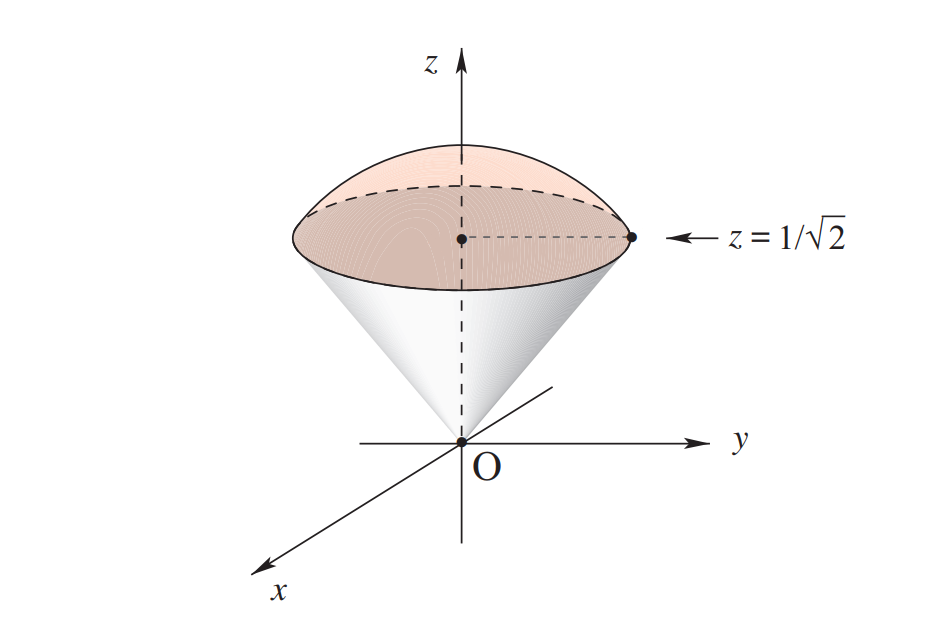
\includegraphics[width=0.4\textwidth]{Pictures/Tutorial 7-1.png}
        \caption{Area of the portion of the unit sphere enclosed by the cone \(z \geq \sqrt{x^2 + y^2}\).}
    \end{figure}
    
    Recall that the parametrization of the surface area of the unit sphere is given by:
    \begin{align}
        \Phi(\theta, \phi) &= (x, y, z) \\
        &= (\cos(\theta)\sin(\phi), \sin(\theta)\sin(\phi), \cos(\phi))
    \end{align}
    where \(0 \leq \theta \leq 2\pi\) and \(0 \leq \phi \leq \pi\).
    
    Since we want to find the surface area of the sphere enclosed by the cone, we must first find the bounds of our integral in terms of \(\theta\) and \(\phi\).
    
    From the figure, observe that \(0 \leq \theta < 2\pi\). The bounds for the angle \(\theta\) remain unchanged.
    
    However, observe also that:
    \begin{align*}
        \frac{1}{\sqrt{2}} \leq & \ z \leq 1 \\
        \frac{1}{\sqrt{2}} \leq & \ \cos(\phi) \leq 1
    \end{align*}
    
    We find that \(0 \leq \phi \leq \frac{\pi}{4}\).
    
    Recall that the area of a parametrized surface is given by:
    \begin{align}
        A(S) &= \iint_D \|\Phi_u \times \Phi_v \| \ dudv
    \end{align}
    
    We know from spherical coordinates that the norm of the cross product is equal to the Jacobian:
    \begin{align}
        \|\Phi_\theta \times \Phi_\phi \| &= \left|\frac{\partial(x, y, z)}{\partial(\rho, \theta, \phi)}\right| \\
        &= \rho^2\sin(\phi)
    \end{align}
    
    Since \(\rho = 1\), we have that:
    \begin{align*}
        \|\Phi_\theta \times \Phi_\phi \| &= \sin(\phi)
    \end{align*}
    
    Then the surface area of the sphere enclosed by the cone is given by:
    \begin{align*}
        A(S) &= \iint_D \|\Phi_\theta \times \Phi_\phi \| \ d\theta d\phi \\
        &= \int_0^{\frac{\pi}{4}} \int_0^{2\pi} \sin(\phi) \ d\theta d\phi \\
        &= 2\pi \int_0^{\frac{\pi}{4}} \sin(\phi) \ d\phi \\
        &= -2\pi \cos(\phi) \Big|_0^{\frac{\pi}{4}} \\
        &= -2\pi \cos\left(\frac{\pi}{4}\right) + 2\pi \cos(0)  \\
        &= -\frac{2\pi}{\sqrt{2}} + 2\pi \\
        &= 2\pi\left(1 -\frac{1}{\sqrt{2}}\right)
    \end{align*}
\end{solution}

\newpage 

\setcounter{section}{8}
\section{\centering Tutorial 8}

\subsection{Section 7.5}

\begin{tcolorbox}[
        title={Problem 6},
        valign=center,
        nobeforeafter,
        colframe=gray!95!black
    ]
    Evaluate the integral:
    \begin{align}
        \iint_S x^2z + y^2z \ dS
    \end{align}
    where \(S\) is the part of the plane \(z = 4 + x + y\) that lies inside the cylinder \(x^2 + y^2 = 4\).
\end{tcolorbox}

\begin{solution}
    The plane is restricted to inside of a cylinder. The surface \(S\) is then best parametrized in cylindrical coordinates. 
    
    Recall cylindrical coordinates:
    \begin{align}
        x &= r\cos(\theta) & y &= r\sin(\theta) & z &= z
    \end{align}
    
    The plane is then given by:
    \begin{align*}
        z &= 4 + x + y \\
        &= 4 + r \cos(\theta) + r \sin(\theta)
    \end{align*}
    
    The domain of integration is restricted to \(D = \{(x, y) \in \mathbb{R}^2 \ | \ x^2 + y^2 \leq 2^2\}\):
    \begin{align*}
        x^2 + y^2 &\leq 2^2 \\
        r^2 &\leq 2^2 \\
        r &\leq 2
    \end{align*}
    
    We therefore have the following parametrization for the surface \(S\):
    \begin{align}
        \Phi(r, \theta) &= \left(x, y, z\right) \\
        &= \left(r\cos(\theta), r\sin(\theta), 4 + r\cos(\theta) + r\sin(\theta)\right)
    \end{align}
    where \(0 \leq r \leq 2\) and \(0 \leq \theta \leq 2\pi\).
    
    We first compute the partial derivatives:
    \begin{align*}
        \Phi_r &= \left(\cos(\theta), \sin(\theta), \cos(\theta) + \sin(\theta)\right) & \Phi_\theta &= \left(-r\sin(\theta), r\cos(\theta), -r\sin(\theta) + r\cos(\theta)\right)
    \end{align*}
    
    We now compute the Jacobian:
    \begin{align*}
        \|\Phi_r \times \Phi_\theta\| &= \|\left(\cos(\theta), \sin(\theta), \cos(\theta) + \sin(\theta)\right) \times \left(-r\sin(\theta), r\cos(\theta), -r\sin(\theta) + r\cos(\theta)\right) \| \\
        &= \|\left(- r\sin^2(\theta) - r\cos^2(\theta), - r\sin^2(\theta) - r\cos^2(\theta), r\cos^2(\theta) + r\sin^2(\theta)\right) \| \\
        &= \|\left(- r, - r, r\right) \| \\
        &= \sqrt{r^2 + r^2 + r^2} \\
        &= r\sqrt{3}
    \end{align*}
    
    We now evaluate the integral:
    \begin{align*}
        \iint_S x^2z + y^2z \ dS &= \iint_S (x^2 + y^2)z \ dS \\
        &= \iint_D r^2(4 + r\cos(\theta) + r\sin(\theta)) \|\Phi_r \times \Phi_\theta\| \ dr d\theta \\
        &= \iint_D r^2(4 + r\cos(\theta) + r\sin(\theta)) r\sqrt{3} \ dr d\theta \\
        &= \sqrt{3}\int_0^{2\pi} \int_0^2 4r^3 + r^4\left(\cos(\theta) + \sin(\theta)\right) \ drd\theta \\
        &= \sqrt{3}\int_0^{2\pi} r^4\Big|_0^2 + \frac{r^5}{5}\left(\cos(\theta) + \sin(\theta)\right)\Biggr|_0^2 \ d\theta \\
        &= \sqrt{3}\int_0^{2\pi} 16 + \frac{32}{5}\left(\cos(\theta) + \sin(\theta)\right) \ d\theta \\
        &= \sqrt{3}\left( 16 \theta + \frac{32}{5}\left(\sin(\theta) - \cos(\theta)\right)\right) \Biggr|_0^{2\pi} \\\
        &= \sqrt{3}\left( 16 (2\pi)\right) \\
        &= 32 \pi \sqrt{3}
    \end{align*}
\end{solution}

\begin{tcolorbox}[
        title={Problem 17},
        valign=center,
        nobeforeafter,
        colframe=gray!95!black
    ]
    Let \(S\) be a sphere of radius \(R\). \\
    
    Argue by symmetry that:
    \begin{align}
        \iint_S x^2 \ dS = \iint_S y^2 \ dS = \iint_S z^2 \ dS
    \end{align}
    
    Use this fact to evaluate, with very little computation, the integral:
    \begin{align}
        \iint_S x^2 \ dS
    \end{align}
\end{tcolorbox}

\begin{solution}
    Since spheres are symmetric with respect to the \(xy\), \(xz\), and \(yz\) planes, interchanging the variables \(x\), \(y\), and \(z\) in the integral will not affect the value of the integral.
    
    We now evaluate:
    \begin{align}
        \iint_S x^2 \ dS
    \end{align}
    
    Recall spherical coordinates on a sphere of radius \(R\):
    \begin{align}
        x &= R\cos(\theta) \sin(\varphi) & y &= R\sin(\theta) \sin(\varphi) & z &= R\cos(\varphi) & x^2 + y^2 + z^2 &= R^2
    \end{align}
    
    Observe that:
    \begin{align*}
        \iint_S x^2 \ dS &= \iint_S \frac{x^2 + x^2 + x^2}{3} \ dS \\
        &= \iint_S \frac{x^2 + y^2 + z^2}{3} \ dS \\
        &= \frac{1}{3} \iint_S x^2 + y^2 + z^2 \ dS \\
        &= \frac{1}{3} \iint_S R^2 \ dS \\
        &= \frac{R^2}{3} \iint_S dS \\
        &= \frac{R^2}{3} (4\pi R^2) \\
        &= \frac{4\pi R^4}{3}
    \end{align*}
    where we used the fact that the total surface area of a sphere of radius \(R\) is equal to \(4\pi R^2\). 
\end{solution}

\subsection{Section 7.6}

\begin{tcolorbox}[
        title={Problem 9},
        valign=center,
        nobeforeafter,
        colframe=gray!95!black
    ]
    Let \(\vb{F} = y\vb{i} - x\vb{j} + x^3y^2z\vb{k}\). \\
    
    Evaluate:
    \begin{align}
        \iint_S (\nabla \times \vb{F}) \cdot d\vb{S}
    \end{align}
    where \(S\) is the surface \(x^2 + y^2 + 3z^2 = 1\) and \(z \leq 0\), oriented by the upward-pointing normal.
\end{tcolorbox}

\begin{solution}
    \textit{(The long way around)}

    Let \(D\) denote the unit disk:
    \begin{align}
        D &= \{(x, y) \in \mathbb{R}^2 \ | \ x^2 + y^2 \leq 1\}
    \end{align}
    
    Observe that, since the surface \(S\) lies below the \(xy\) plane, it can be parametrized as a graph \(z = g(x, y)\) over \(D\) given by:
    \begin{align}
        g(x, y) &= - \sqrt{\frac{1 - x^2 - y^2}{3}}
    \end{align}

    We first compute the partial derivatives of \(g\):
    \begin{align*}
        \frac{\partial g}{\partial x} &= \frac{x}{\sqrt{3(1 - x^2 - y^2)}} & \frac{\partial g}{\partial y} &= \frac{y}{\sqrt{3(1 - x^2 - y^2)}}
    \end{align*}

    We now calculate the curl of \(\vb{F}\):
    \begin{align*}
        \nabla \times \vb{F} &= 
        \begin{vmatrix}
            \vb{i} & \vb{j} & \vb{k} \\
            \frac{\partial}{\partial x} & \frac{\partial}{\partial y} & \frac{\partial}{\partial z} \\
            y & -x & zx^3y^2
        \end{vmatrix} \\
        &= \left(\frac{\partial (x^3y^2z)}{\partial y} - \frac{\partial (-x)}{\partial z}\right)\vb{i} + \left(\frac{\partial (y)}{\partial z} - \frac{\partial (x^3y^2z)}{\partial x}\right)\vb{j} + \left(\frac{\partial (-x)}{\partial x} - \frac{\partial (y)}{\partial y}\right)\vb{k} \\
        &= 2x^3yz\vb{i} - 3x^2y^2z\vb{j} -2\vb{k}
    \end{align*}

    We now evaluate the integral with \(z = g(x, y)\):
    \begin{align*}
        \iint_S \nabla \times \vb{F} \cdot d\vb{S} &= \iint_D \nabla \times \vb{F} \cdot (-g_x, -g_y, 1) \ dxdy \\
        &= \iint_D \left(2x^3yz, - 3x^2y^2z, -2\right) \cdot (-g_x, -g_y, 1) \ dxdy \\
        &= \iint_D -2x^3y z g_x + 3x^2y^2 z g_y -2 \ dxdy \\
        &= \iint_D 2x^3y \sqrt{\frac{1 - x^2 - y^2}{3}} \frac{x}{\sqrt{3(1 - x^2 - y^2)}} \\
        &\quad - 3x^2y^2 \sqrt{\frac{1 - x^2 - y^2}{3}} \frac{y}{\sqrt{3(1 - x^2 - y^2)}} -2 \ dxdy \\
        &= \iint_D \frac{2}{3}x^4y - x^2y^3 - 2 \ dxdy
    \end{align*}
    
    Now, recall polar coordinates:
    \begin{align}
        x &= r\cos(\theta) & y &= r\sin(\theta) & dxdy &= r \ dr d\theta
    \end{align}
    
    Then the integral is given by:
    \begin{align*}
        \iint_S \nabla \times \vb{F} \cdot d\vb{S} &= \iint_D \frac{2}{3}x^4y - x^2y^3 - 2 \ dxdy \\
        &= \int_0^1 \int_0^{2\pi} \left(\frac{2}{3}\left(r\cos(\theta)\right)^4\left(r\sin(\theta)\right) - \left(r\cos(\theta)\right)^2\left(r\sin(\theta)\right)^3 - 2\right) r \ d\theta dr \\
        &= \int_0^1 \int_0^{2\pi} \frac{2}{3}r^6\cos^4(\theta)\sin(\theta) - r^6\cos^2(\theta)\sin^3(\theta) - 2r \ d\theta dr \\
        &= \int_0^1 \int_0^{2\pi} \frac{2}{3}r^6\cos^4(\theta)\sin(\theta) \ d\theta dr - \int_0^1 \int_0^{2\pi} r^6\cos^2(\theta)\sin^3(\theta) \ d\theta dr \\
        &\quad - 2 \int_0^1 \int_0^{2\pi} r \ d\theta dr
    \end{align*}
    
    To solve this integral faster, we make use of an important identity. For all \(n\), \(m \in \mathbb{Z}\):
    \begin{align}
        \int_0^{2\pi} \sin^{2m+1}(x)\cos^n(x) \ dx &= 0 & \int_0^{2\pi} \sin^{m}(x)\cos^{2n+1}(x) \ dx &= 0
    \end{align}
    
    This follows from the fact that we are integrating over a full period. You should convince yourself that this makes sense before you use it.
    
    Then:
    \begin{align*}
        \iint_S \nabla \times \vb{F} \cdot d\vb{S} &= \int_0^1 \int_0^{2\pi} \frac{2}{3}r^6\cos^4(\theta)\sin(\theta) \ d\theta dr - \int_0^1 \int_0^{2\pi} r^6\cos^2(\theta)\sin^3(\theta) \ d\theta dr \\
        &\quad - 2 \int_0^1 \int_0^{2\pi} r \ d\theta dr \\
        &= - 2 \int_0^1 \int_0^{2\pi} r \ d\theta dr \\
        &= -4\pi \int_0^1 r \ dr \\
        &= -4\pi \frac{r^2}{2}\Biggr|_0^1 \\
        &= -2\pi 
    \end{align*}
\end{solution}

\begin{solution}
    \textit{(Stokes' Theorem)}

    You can visualize the surface \(S\) as a bowl lying below the \(xy\) plane. 
    
    Observe then that the boundary of the surface \(S\) is the unit circle lying on the \(xy\) plane:
    \begin{align}
        \partial S &= \{(x, y, z) \in \mathbb{R}^3 \ | \ x^2 + y^2 = 1, z = 0\}
    \end{align}

    Since the normal of the surface \(S\) points upwards, the orientation for this curve must be counter-clockwise.

    We may then parametrize this boundary by:
    \begin{align}
        \vb{c}(t) &= (\cos(t), \sin(t), 0)
    \end{align}
    where \(0 \leq t \leq 2\pi\).
    
    Observe that \(\vb{F}\) has no singularities on \(S\).
    
    Then by Stokes' Theorem:
    \begin{align*}
        \iint_S \nabla \times \vb{F} \cdot d \vb{S} &= \oint_{\partial S} \vb{F} \cdot d\vb{s} \\
        &= \int_{0}^{2\pi} \vb{F}(\vb{c}(t)) \cdot \vb{c}'(t) \ dt \\
        &= \int_{0}^{2\pi} (\sin(t), -\cos(t), 0) \cdot (-\sin(t), \cos(t), 0) \ dt \\
        &= \int_{0}^{2\pi} -\sin^2(t) - \cos^2(t) \ dt \\
        &= -\int_{0}^{2\pi} dt \\
        &= -2\pi
    \end{align*}
\end{solution}

\begin{tcolorbox}[
        title={Problem 11},
        valign=center,
        nobeforeafter,
        colframe=gray!95!black
    ]
    Let \(\vb{F} = (x + 3y^5) \vb{i} + (y + 10xz) \vb{j} + (z - xy) \vb{k}\). \\
    
    Calculate the integral:
    \begin{align}
        \iint_S \vb{F} \cdot d\vb{S}
    \end{align}
    where \(S\) is the entire surface of the solid half ball \(x^2 + y^2 + z^2 \leq 1\) and \(z \geq 0\), oriented by the outward-pointing normal (including the \(z = 0\) disk).
\end{tcolorbox}

\begin{solution}
    \textit{(The long way around)} 
    
    We split the surface integral into two parts: the flux of \(\vb{F}\) across the upper hemisphere \(S_1\) and the flux of \(\vb{F}\) across the disk \(S_2\).
    \begin{align}
        \iint_S \vb{F} \cdot d\vb{S} &= \iint_{S_1} \vb{F} \cdot d\vb{S} + \iint_{S_2} \vb{F} \cdot d\vb{S}
    \end{align}
    
    First, recall spherical coordinates on a unit sphere (\(R = 1\)):
    \begin{align}
        x &= \cos(\theta) \sin(\varphi) & y &= \sin(\theta) \sin(\varphi) & z &= \cos(\varphi) & dS &= \sin(\varphi) \ d\theta d\varphi
    \end{align}
    \begin{align}
        x^2 + y^2 + z^2 = 1^2
    \end{align}
    
    Then the flux across the upper hemisphere is given by:
    \begin{align*}
        \iint_{S_1} \vb{F} \cdot d\vb{S} &= \iint_{S_1} \vb{F} \cdot \vb{\hat{n}} \ dS \\
        &= \iint_{S_1} \vb{F} \cdot \vb{\hat{r}} \ dS \\
        &= \iint_{S_1} \left(x + 3y^5, y + 10xz, z - xy\right) \cdot \left(x, y, z\right) \ dS \\
        &= \iint_{S_1} x^2 + 3xy^5 + y^2 + 10xyz + z^2 - xyz \ dS \\
        &= \iint_{S_1} x^2 + y^2 + z^2 + 3xy^5 + 9xyz \ dS \\
    \end{align*}
    
    Since the surface \(S_1\) has a radius of 1, we may simplify \(x^2 + y^2 + z^2 = 1\):
    \begin{align*}
        \iint_{S_1} \vb{F} \cdot d\vb{S} &= \iint_{S_1} 1 + 3xy^5 + 9xyz \ dS \\
        &= \iint_{S_1} 1 + 3\cos(\theta) \sin(\varphi)\sin^5(\theta) \sin^5(\varphi) + 9\cos(\theta) \sin(\varphi)\sin(\theta) \sin(\varphi)\cos(\varphi) \ dS \\
        &= \iint_{S_1} 1 + 3\cos(\theta)\sin^5(\theta)\sin^6(\varphi) + 9\cos(\theta)\sin(\theta) \cos(\varphi)\sin^2(\varphi) \ dS \\
        &= \int_{0}^{\frac{\pi}{2}} \int_0^{2\pi} \left(1 + 3\cos(\theta)\sin^5(\theta)\sin^6(\varphi) + 9\cos(\theta)\sin(\theta) \cos(\varphi)\sin^2(\varphi)\right) \sin(\varphi) \ d\theta d\varphi \\
        &= \int_{0}^{\frac{\pi}{2}} \int_0^{2\pi} \sin(\varphi) + 3\cos(\theta)\sin^5(\theta)\sin^7(\varphi) + 9\cos(\theta)\sin(\theta) \cos(\varphi)\sin^3(\varphi) \ d\theta d\varphi \\
        &= \int_{0}^{\frac{\pi}{2}} \left( \sin(\varphi) \theta - 3\frac{\cos^6(\theta)}{6}\sin^7(\varphi) + 9\frac{\sin^2(\theta)}{2} \cos(\varphi)\sin^3(\varphi)\right)\Biggr|_0^{2\pi} \ d\varphi \\
        &= \int_{0}^{\frac{\pi}{2}} 2\pi\sin(\varphi) + 0 + 0 \ d\varphi \\
        &= 2\pi\int_{0}^{\frac{\pi}{2}} \sin(\varphi) \ d\varphi \\
        &= - 2\pi \cos(\varphi) \Big|_0^{\frac{\pi}{2}} \\
        &= - 2\pi \cos\left(\frac{\pi}{2}\right) + 2\pi \cos(0) \\
        &= 2\pi
    \end{align*}
    
    Now, recall polar coordinates:
    \begin{align}
        x &= r \cos(\theta) & y &= r \sin(\theta) & dA &= r \ dr d\theta
    \end{align}
    
    Then the flux across the disk is given by:
    \begin{align*}
        \iint_{S_2} \vb{F} \cdot d\vb{S} &= \iint_{S_2} \vb{F} \cdot \vb{\hat{n}} \ dS \\
        &= \iint_{S_2} (x + 3y^5) \vb{i} + (y + 10xz) \vb{j} + (z - xy) \vb{k} \cdot (-\vb{k}) \ dS \\
        &= \iint_{S_2} -(z - xy) \ dS
    \end{align*}
    where \(\vb{\hat{n}} = -\vb{k}\) is the outward-pointing normal relative to the solid half ball.
    
    Since the surface \(S_2\) lies on the \(z = 0\) plane, we must evaluate \(\vb{F}\) at \(z = 0\):
    \begin{align*}
        \iint_{S_2} \vb{F} \cdot d\vb{S} &= \iint_{S_2} -z + xy \ dS \\
        &= \iint_{S_2} xy \ dS \\
        &= \iint_{D_2} xy \ dA \\
        &= \int_{0}^{2\pi} \int_0^1 r\cos(\theta) r\sin(\theta) r \ drd\theta \\
        &= \int_{0}^{2\pi} \int_0^1 r^3\cos(\theta) \sin(\theta) \ drd\theta \\
        &= \int_{0}^{2\pi} \frac{r^4}{4} \Biggr|_0^1 \cos(\theta) \sin(\theta) \ d\theta \\
        &= \frac{1}{4} \int_{0}^{2\pi} \cos(\theta) \sin(\theta) \ d\theta \\
        &= \frac{1}{4} \frac{\sin^2(\theta)}{2}\Biggr|_{0}^{2\pi} \\
        &= 0
    \end{align*}
    
    Then the total flux of \(\vb{F}\) across \(S\) is given by:
    \begin{align*}
        \iint_S \vb{F} \cdot d\vb{S} &= \iint_{S_1} \vb{F} \cdot d\vb{S} + \iint_{S_2} \vb{F} \cdot d\vb{S} \\
        &= 2\pi + 0 \\
        &= 2\pi
    \end{align*}
\end{solution}

\begin{solution}
    \textit{(Divergence Theorem)}
    
    Let the region \(W\) denote the solid half ball:
    \begin{align}
        W &= \{(x, y, z) \in \mathbb{R}^3 \ | \ x^2 + y^2 + z^2 \leq 1, \ z \geq 0\}
    \end{align} 
    
    It follows then that
    \begin{align}
        S &= \partial W
    \end{align}

    Observe that \(\vb{F}\) has no singularities in \(W\).

    Then by the Divergence Theorem:
    \begin{align*}
        \iint_S \vb{F} \cdot \ d\vb{S} &= \iiint_W \nabla \cdot \vb{F} \ dV \\
        &= \iiint_W \nabla \cdot \left(x + 3y^5, y + 10xz, z - xy\right) \ dV \\
        &= \iiint_W 1 + 1 + 1 \ dV \\
        &= 3 \iiint_W dV \\
        &= 3 \left(\frac{1}{2}\frac{4\pi}{3}\right) \\
        &= 2\pi
    \end{align*}
    where we used the fact that the volume of a sphere of radius \(R\) is equal to \(\frac{4\pi R^3}{3}\).
\end{solution}

\newpage 

\setcounter{section}{9}
\section{\centering Tutorial 9}

\subsection{Section 8.1}

\begin{tcolorbox}[
        title={Problem 17},
        valign=center,
        nobeforeafter,
        colframe=gray!95!black
    ]
    Verify Green's Theorem for \(P = 2x^3 - y^3\), \(Q = x^3 + y^3\), and the annular region \(D\) described by \(a \leq x^2 + y^2 \leq b\).
\end{tcolorbox}

We must verify:
\begin{align}
    \int_{\partial D} P \ dx + Q \ dy &= \iint_D \frac{\partial Q}{\partial x} - \frac{\partial P}{\partial y} \ dxdy 
\end{align}
\begin{solution}
    \textit{(Surface integral)}
    
    We first compute the partial derivatives:
    \begin{align*}
        \frac{\partial Q}{\partial x} &= 3x^2 & \frac{\partial P}{\partial y} &= -3y^2
    \end{align*}
    
    We now evaluate the integral:
    \begin{align*}
        \iint_D \frac{\partial Q}{\partial x} - \frac{\partial P}{\partial y} \ dxdy &= \iint_D 3x^2 + 3y^2 \ dxdy 
    \end{align*}
    
    Recall polar coordinates:
    \begin{align*}
        x^2 + y^2 &= r^2 & dxdy &= r \ dr d\theta
    \end{align*}
    
    Then the domain in polar coordinates is given by:
    \begin{align}
        D &= \{(r, \theta) \ | \ \sqrt{a} \leq r \leq \sqrt{b}, \ 0 \leq \theta \leq 2\pi\}
    \end{align}
    
    Then then integral is given by:
    \begin{align*}
        \iint_D \frac{\partial Q}{\partial x} - \frac{\partial P}{\partial y} \ dxdy &= \iint_D 3x^2 + 3y^2 \ dxdy \\
        &= 3\iint_D r^2 r \ dr d\theta \\
        &= 3\int_0^{2\pi} \int_{\sqrt{a}}^{\sqrt{b}} r^3 \ dr d\theta \\
        &= 3\int_0^{2\pi} \frac{r^4}{4} \Biggr|_{\sqrt{a}}^{\sqrt{b}} \ d\theta \\
        &= \frac{3}{4}(b^2 - a^2) \int_0^{2\pi} d\theta \\
        &= \frac{3\pi}{2}(b^2 - a^2)
    \end{align*}
\end{solution}

\begin{solution}
    \textit{(Line integral)}
    
    Observe that the boundary of the domain \(D\) is the circle of radius \(\sqrt{a}\) and the circle of radius \(\sqrt{b}\):
    \begin{align}
        \partial D &= \{(x, y) \in \mathbb{R}^2 \ | \ x^2 + y^2 = a\} \cup \{(x, y) \in \mathbb{R}^2 \ | \ x^2 + y^2 = b\}
    \end{align}
    
    In order for the domain \(D\) to remain on the left as you traverse along the curves, the inner circle must be oriented clockwise and the outer circle must be oriented counter-clockwise relative to the \(xy\) plane.
    
    We may then parametrize these boundary segments respectively by:
    \begin{align}
        \vb{c}_1(t) &= \left(\sqrt{a}\cos(t), \sqrt{a}\sin(t)\right) & \vb{c}_2(t) &= \left(\sqrt{b}\cos(t), \sqrt{b}\sin(t)\right)
    \end{align}
    where \(0 \leq t \leq 2\pi\).
    
    We now evaluate the integral:
    \begin{align*}
        \int_{\partial D} P \ dx + Q \ dy &= \int_{\partial D} (P, Q) \ (dx, dy) \\ 
        &= \int_{\partial D} (2x^3 - y^3, x^3 + y^3) \cdot d\vb{s} \\ 
        &= \int_{C_1} (2x^3 - y^3, x^3 + y^3) \cdot d\vb{s} + \int_{C_2} (2x^3 - y^3, x^3 + y^3) \cdot d\vb{s} \\
        &= \int_0^{-2\pi} \left(2\sqrt{a^3}\cos^3(t) - \sqrt{a^3}\sin^3(t), \sqrt{a^3}\cos^3(t) + \sqrt{a^3}\sin^3(t)\right) \cdot \vb{c}'_1(t) \ dt \\
        &\quad + \int_0^{2\pi} \left(2\sqrt{b^3}\cos^3(t) - \sqrt{b^3}\sin^3(t), \sqrt{b^3}\cos^3(t) + \sqrt{b^3}\sin^3(t)\right) \cdot \vb{c}'_2(t) \ dt \\
        &= \int_0^{-2\pi} \left(2\sqrt{a^3}\cos^3(t) - \sqrt{a^3}\sin^3(t), \sqrt{a^3}\cos^3(t) + \sqrt{a^3}\sin^3(t)\right) \cdot \left(-\sqrt{a}\sin(t), \sqrt{a}\cos(t)\right) \ dt \\
        &\quad + \int_0^{2\pi} \left(2\sqrt{b^3}\cos^3(t) - \sqrt{b^3}\sin^3(t), \sqrt{b^3}\cos^3(t) + \sqrt{b^3}\sin^3(t)\right) \cdot \left(-\sqrt{b}\sin(t), \sqrt{b}\cos(t)\right) \ dt \\
        &= \int_0^{-2\pi} -2a^2\cos^3(t)\sin(t) + a^2\sin^4(t) + a^2\cos^4(t) + a^2\sin^3(t)\cos(t) \ dt \\
        &\quad + \int_0^{2\pi} -2b^2\cos^3(t)\sin(t) +b^2\sin^4(t) + b^2\cos^4(t) + b^2\sin^3(t)\cos(t) \ dt \\
        &= \int_0^{-2\pi} -2a^2\cos^3(t)\sin(t) + a^2\sin^4(t) + a^2\cos^4(t) + a^2\sin^3(t)\cos(t) \ dt \\
        &\quad + \int_0^{2\pi} -2b^2\cos^3(t)\sin(t) +b^2\sin^4(t) + b^2\cos^4(t) + b^2\sin^3(t)\cos(t) \ dt \\
        &= -\frac{3\pi}{2}a^2 + \frac{3\pi}{2}b^2 \\
        &= \frac{3\pi}{2}(b^2 - a^2)
    \end{align*}
    by WolframAlpha.
    
    Then we have verified Green's Theorem for this specific example.
\end{solution}

\begin{tcolorbox}[
        title={Problem 24},
        valign=center,
        nobeforeafter,
        colframe=gray!95!black
    ]
    If \(C\) is a simple, closed curve that bounds a region to which Green’s Theorem applies, then the area of the region \(D\) bounded by \(C = \partial D \) is given by:
    \begin{align}
        A &= \frac{1}{2} \int_{\partial D} x \ dy - y \ dx
    \end{align}
    
    Use the above statement to recover the formula:
    \begin{align}
        A &= \frac{1}{2} \int_a^b r^2 \ d\theta
    \end{align}
    for a region in polar coordinates.
\end{tcolorbox}

\begin{solution}
    Recall Green's Theorem:
    \begin{align}
        \int_{\partial D} P \ dx + Q \ dy &= \iint_D \frac{\partial Q}{\partial x} - \frac{\partial P}{\partial y} \ dxdy
    \end{align}
    
    Observe that by Green's Theorem:
    \begin{align*}
        A &= \frac{1}{2} \int_{\partial D} x \ dy - y \ dx \\
        &= \frac{1}{2} \int_{\partial D} - y \ dx + x \ dy \\
        &= \frac{1}{2} \iint_{D} \frac{\partial x}{\partial x} - \frac{\partial (-y)}{\partial y} \ dxdy \\
        &= \frac{1}{2} \iint_{D} 1 + 1 \ dxdy \\
        &= \frac{1}{2} \iint_{D} 2 \ dxdy \\
        &= \iint_{D} dA
    \end{align*}

    Recall polar coordinates:
    \begin{align}
        dA &= r \ dr d\theta
    \end{align}

    Then, for an arbitrary region \(D\):
    \begin{align*}
        A &= \iint_{D} dA \\
        &= \int_{a}^{b} \int_0^r r \ dr d\theta \\
        &= \int_{a}^{b} \frac{r^2}{2} \Biggr|_0^r \ d\theta \\
        &= \frac{1}{2} \int_{a}^{b} r^2 \ d\theta
    \end{align*}
    where the radial direction \(r\) may or may not depend on \(\theta\), and \(a \leq \theta \leq b\) for arbitrary angles \(a\) and \(b\).
\end{solution}

\subsection{Section 8.2}

\begin{tcolorbox}[
        title={Problem 17},
        valign=center,
        nobeforeafter,
        colframe=gray!95!black
    ]
    Calculate the surface integral:
    \begin{align}
        \iint_S \nabla \times \vb{F} \cdot d\vb{S}
    \end{align}
    where \(S\) is the hemisphere \(x^2 + y^2 + z^2 = 1\) where \(x \geq 0\), and \(\vb{F} = x^3 \vb{i} - y^3 \vb{j}\).
\end{tcolorbox}

\begin{solution}
    \textit{(Surface integral)}
    
    We first compute the curl of \(\vb{F}\):
    \begin{align*}
        \nabla \times \vb{F} &= \vb{0}
    \end{align*}
    
    Then, trivially:
    \begin{align*}
        \iint_S \nabla \times \vb{F} \cdot d\vb{S} &= \iint_S \vb{0} \cdot d\vb{S} \\
        &= 0
    \end{align*}
\end{solution}

\begin{solution}
    \textit{(Line integral)}
    
    Observe then that the boundary of the surface \(S\) is the unit circle lying on the \(yz\) plane:
    \begin{align}
        \partial S &= \{(x, y, z) \in \mathbb{R}^3 \ | \ y^2 + z^2 = 1, x = 0\}
    \end{align}

    Since the normal of the surface \(S\) points outwards, the orientation for this curve must be clockwise relative to the \(yz\) plane.

    We may then parametrize this boundary by:
    \begin{align}
        \vb{c}(t) &= (0, \cos(t), \sin(t))
    \end{align}
    where \(0 \leq t \leq 2\pi\).
    
    Observe that \(\vb{F}\) has no singularities on \(S\).
    
    Then by Stokes' Theorem:
    \begin{align*}
        \iint_S \nabla \times \vb{F} \cdot d \vb{S} &= \oint_{\partial S} \vb{F} \cdot d\vb{s} \\
        &= \int_{2\pi}^{0} \vb{F}(\vb{c}(t)) \cdot \vb{c}'(t) \ dt \\
        &= \int_{2\pi}^{0} (0, -\cos^3(t), 0) \cdot (0, -\sin(t), \cos(t)) \ dt \\
        &= \int_{2\pi}^{0} \cos^3(t)\sin(t) \ dt \\
        &= - \frac{\cos^4(x)}{4} \Biggr|_{2\pi}^{0} \\
        &= 0
    \end{align*}
\end{solution}

\begin{tcolorbox}[
        title={Problem 29},
        valign=center,
        nobeforeafter,
        colframe=gray!95!black
    ]
    Verify Stokes' Theorem for the helicoid
    \begin{align}
        \Phi(r, \theta) &= (r \cos(\theta), r\sin(\theta), \theta)
    \end{align}
    where \((r, \theta) \in [0, 1] \times \left[0, \frac{\pi}{2}\right]\), and \(\vb{F}(x, y, z) = (z, x, y)\).
\end{tcolorbox}

We must verify:
\begin{align}
    \int_{\partial S} \vb{F} \cdot d\vb{s} &= \iint_S \nabla \times \vb{F} \cdot d\vb{S}
\end{align}

\begin{solution}
    \textit{(Surface integral)}
    
    We first compute the curl of \(\vb{F}\):
    \begin{align*}
        \nabla \times \vb{F} &= (1, 1, 1)
    \end{align*}
    
    We now compute the partial derivatives of \(\Phi\):
    \begin{align*}
        \Phi_r &= (\cos(\theta), \sin(\theta), 0) & \Phi_\theta &= (-r \sin(\theta), r\cos(\theta), 1)
    \end{align*}
    
    We now compute the cross product \(\Phi_r \times \Phi_\theta\):
    \begin{align*}
        \Phi_r \times \Phi_\theta &= (\sin(\theta), -\cos(\theta), r)
    \end{align*}
    
    We now evaluate the integral:
    \begin{align*}
        \iint_S \nabla \times \vb{F} \cdot d\vb{S} &= \iint_D \left(\nabla \times \vb{F}\right) \cdot \left(\Phi_r \times \Phi_\theta\right) \ dr d\theta \\
        &= \int_0^{\frac{\pi}{2}} \int_0^1 \left(1, 1, 1\right) \cdot (\sin(\theta), -\cos(\theta), r) \ dr d\theta \\
        &= \int_0^{\frac{\pi}{2}} \int_0^1 \sin(\theta) - \cos(\theta) + r \ dr d\theta \\
        &= \int_0^{\frac{\pi}{2}} \left(r\sin(\theta) - r\cos(\theta) + \frac{r^2}{2}\right) \Biggr|_0^1 \ d\theta \\
        &= \int_0^{\frac{\pi}{2}} \sin(\theta) - \cos(\theta) + \frac{1}{2} \ d\theta \\
        &= \left( -\cos(\theta) - \sin(\theta) + \frac{\theta}{2}\right) \Biggr|_0^{\frac{\pi}{2}} \\
        &= 0 + 0 + \frac{\pi}{4} \\
        &= \frac{\pi}{4}
    \end{align*}
\end{solution}

\begin{solution}
    \textit{(Line integral)}
    
    Observe that the boundary of \(D\) is given by:
    \begin{align*}
        \partial D &= \left\{r = 0, \ 0 \leq \theta \leq \frac{\pi}{2}\right\} \cup \left\{r = 1, \ 0 \leq \theta \leq \frac{\pi}{2}\right\} \cup \left\{0 \leq r \leq 1, \ \theta = 0\right\} \cup \left\{0 \leq r \leq 1, \ \theta = \frac{\pi}{2} \right\}
    \end{align*}
    
    In order for the domain D to remain on the left as you traverse along the curves, the boundary must be traversed counter-clockwise relative to the \(r\theta\) plane.
    
    We may then parametrize these boundary segments respectively by:
    \begin{align*}
        \vb{c}_1(t) &= \left(t, 0\right) & \vb{c}_2(t) &= \left(1, \frac{\pi}{2}t\right) \\
        \vb{c}_3(t) &= \left(1 - t, \frac{\pi}{2}\right) & \vb{c}_4(t) &= \left(0, \frac{\pi}{2}(1 - t)\right)
    \end{align*}
    where \(0 \leq t \leq 1\).
    
    Other parametrizations are equally valid. Note, however, that this parametrization is in terms of \(r\) and \(\theta\).
    
    To find our parametrization in terms of \(x\), \(y\), and \(z\) (this is required because of our vector field \(\vb{F}\)), we must use our initial parametrization \(\Phi\):
    \begin{align*}
        \Phi(\vb{c}_1(t)) &= (t \cos(0), t\sin(0), 0) & \Phi(\vb{c}_2(t)) &= \left( \cos\left(\frac{\pi}{2}t\right), \sin\left(\frac{\pi}{2}t\right), \frac{\pi}{2}t\right) \\
        &= (t, 0, 0) \\
        \\
        \Phi(\vb{c}_3(t)) &= \left(0, (1 - t), \frac{\pi}{2}\right) & \Phi(\vb{c}_4(t)) &= \left(0, 0, \frac{\pi}{2}(1 - t)\right)
    \end{align*}
    
    We now evaluate the integral:
    \begin{align*}
        \int_{\partial D} \vb{F} \cdot d\vb{s} &= \int_{\partial D} (z, x, y) \cdot d\vb{s} \\
        &= \int_{\partial D} (\theta, r\cos(\theta), r\sin(\theta)) \cdot d\vb{s} \\
        &= \int_{C_1} (\theta, r\cos(\theta), r\sin(\theta)) \cdot d\vb{s} + \int_{C_2} (\theta, r\cos(\theta), r\sin(\theta)) \cdot d\vb{s} \\
        &\quad + \int_{C_3} (\theta, r\cos(\theta), r\sin(\theta)) \cdot d\vb{s} + \int_{C_4} (\theta, r\cos(\theta), r\sin(\theta)) \cdot d\vb{s} \\
        &= \int_0^1 (0, t\cos(0), t\sin(0)) \cdot \Phi'(\vb{c}_1(t)) \ dt + \int_0^1 \left(\frac{\pi}{2}t, \cos\left(\frac{\pi}{2}t\right), \sin\left(\frac{\pi}{2}t\right)\right) \cdot \Phi'(\vb{c}_2(t)) \ dt \\
        &\quad + \int_0^1 \left(\frac{\pi}{2}, (1 - t)\cos\left(\frac{\pi}{2}\right), (1- t)\sin\left(\frac{\pi}{2}\right)\right) \cdot \Phi'(\vb{c}_3(t)) \ dt + \int_0^1 \left(\frac{\pi}{2}(1 - t), 0, 0\right) \cdot \Phi'(\vb{c}_4(t)) \ dt \\
        &= \int_0^1 (0, t\cos(0), t\sin(0)) \cdot (1, 0, 0) \ dt \\
        &\quad + \int_0^1 \left(\frac{\pi}{2}t, \cos\left(\frac{\pi}{2}t\right), \sin\left(\frac{\pi}{2}t\right)\right) \cdot \left(-\frac{\pi}{2}\sin\left(\frac{\pi}{2}t\right), \frac{\pi}{2}\cos\left(\frac{\pi}{2}t\right), \frac{\pi}{2}\right) \ dt \\
        &\quad + \int_0^1 \left(\frac{\pi}{2}, 0, 1- t\right) \cdot (0, -1, 0) \ dt + \int_0^1 \left(\frac{\pi}{2}(1 - t), 0, 0\right) \cdot \left(0, 0, -\frac{\pi}{2}\right) \ dt \\
        &= \int_0^1 0 \ dt + \int_0^1 \left(\frac{\pi}{2}t, \cos\left(\frac{\pi}{2}t\right), \sin\left(\frac{\pi}{2}t\right)\right) \cdot \left(-\frac{\pi}{2}\sin\left(\frac{\pi}{2}t\right), \frac{\pi}{2}\cos\left(\frac{\pi}{2}t\right), \frac{\pi}{2}\right) \ dt \\
        &\quad + \int_0^1 0 \ dt + \int_0^1 0 \ dt \\
        &= \int_0^1 \left(\frac{\pi}{2}t, \cos\left(\frac{\pi}{2}t\right), \sin\left(\frac{\pi}{2}t\right)\right) \cdot \left(-\frac{\pi}{2}\sin\left(\frac{\pi}{2}t\right), \frac{\pi}{2}\cos\left(\frac{\pi}{2}t\right), \frac{\pi}{2}\right) \ dt \\
        &= \int_0^1 -\frac{\pi^2}{4}t \sin\left(\frac{\pi}{2}t\right) +  \frac{\pi}{2}\cos^2\left(\frac{\pi}{2}t\right) + \frac{\pi}{2}\sin\left(\frac{\pi}{2}t\right) \ dt \\
        &= \frac{\pi}{4}
    \end{align*}
    by WolframAlpha.
    
    Then we have verified Stokes' Theorem for this specific example.
\end{solution}

\newpage 

\setcounter{section}{10}
\section{\centering Tutorial 10}

\subsection{Section 8.3}

\begin{tcolorbox}[
        title={Problem 10 (a)},
        valign=center,
        nobeforeafter,
        colframe=gray!95!black
    ]
    Show that
    \begin{align}
        \vb{F} &= -\frac{\vb{r}}{|\vb{r}|^3}
    \end{align}
    is the gradient of the function \(f(x, y, z) = \frac{1}{r}\).
\end{tcolorbox}

\begin{proof}
\textit{(Cartesian coordinates)}

Recall that the gradient operator in Cartesian coordinates is given by:
\begin{align}
    \nabla &= \left(\frac{\partial}{\partial x}, \frac{\partial}{\partial y}, \frac{\partial}{\partial z}\right)
\end{align}

Then:
\begin{align*}
    \nabla f &= \nabla \left(\frac{1}{r}\right) \\
    &= \nabla \left(\frac{1}{\sqrt{x^2 + y^2 + z^2}}\right) \\
    &= \left(-\frac{2x}{2(x^2 + y^2 + z^2)^{\frac{3}{2}}}, -\frac{2y}{2(x^2 + y^2 + z^2)^{\frac{3}{2}}}, -\frac{2z}{2(x^2 + y^2 + z^2)^{\frac{3}{2}}}\right) \\
    &= \left(-\frac{x}{(x^2 + y^2 + z^2)^{\frac{3}{2}}}, -\frac{y}{(x^2 + y^2 + z^2)^{\frac{3}{2}}}, -\frac{z}{(x^2 + y^2 + z^2)^{\frac{3}{2}}}\right) \\
    &= \left(-\frac{x}{r^3}, -\frac{y}{r^3}, -\frac{z}{r^3}\right) \\
    &= -\frac{\left(x, y, z\right)}{r^{3}} \\
    &= -\frac{\vb{r}}{r^{3}} \\
    &= -\frac{\vb{r}}{|\vb{r}|^{3}} \\
    &=\vb{F}
\end{align*}

Therefore, we have proven that \(\nabla f = \vb{F}\).
\end{proof}

\begin{tcolorbox}[
        title={Problem 10 (b)},
        valign=center,
        nobeforeafter,
        colframe=gray!95!black
    ]
    What is the work done by the force \(\vb{F} = -\frac{\vb{r}}{|\vb{r}|^3}\) in moving a particle from a point \(\vb{r}_0 \in \mathbb{R}^3\) to \(\infty\), where \(\vb{r}(x, y, z) = (x, y, z)\)?
\end{tcolorbox}

\begin{solution}
    Let \(\vb{c}\) be a \(C^1\) curve and let \(f: \mathbb{R}^3 \rightarrow \mathbb{R}\) be a \(C^1\) function. 
    
    Recall by chain rule that:
    \begin{align}
        \frac{d}{dt} f(\vb{c}(t)) &= \nabla f(\vb{c}(t)) \cdot \vb{c}'(t)
    \end{align}
    
    \newpage
    
    Now let \(\vb{c}: [0, 1] \rightarrow \mathbb{R}^3 \backslash (0,0,0)\) be a \(C^1\) curve where \(\vb{c}(0) = \vb{r}_0\) and \(\vb{c}(1) = \vb{r}_1\). Note that we omit the point \((0, 0, 0)\) from our curve since \(\vb{F}(x, y, z)\) is not defined at \((0, 0, 0)\).
    
    The work done by the force \(\vb{F}\) along \(\vb{c}(t)\) is given by:
    \begin{align*}
        W(\vb{r}_0, \vb{r}_1) &= \int_c \vb{F} \cdot d \vb{s} \\
        &= \int_0^1 \vb{F}(\vb{c}(t)) \cdot \vb{c}'(t) \ dt \\
        &= \int_0^1 \nabla f(\vb{c}(t)) \cdot \vb{c}'(t) \ dt \\
        &= \int_0^1 \frac{d}{dt} f(\vb{c}(t)) \ dt \\
        &= f(\vb{c}(1)) - f(\vb{c}(0)) \\
        &= f(\vb{r}_1) - f(\vb{r}_0) \\
        &= \frac{1}{|\vb{r}_1|} - \frac{1}{|\vb{r}_0|} \\
        &= \frac{1}{r_1} - \frac{1}{r_0}
    \end{align*}
    
    Since we want to move the particle from \(\vb{r}_0\) to \(\infty\), let \(r_1 \rightarrow \infty\).
    
    Then:
    \begin{align*}
        W(\vb{r}_0, \infty) &= \lim_{r_1 \rightarrow \infty} \frac{1}{r_1} - \frac{1}{r_0} \\
        &= 0 - \frac{1}{r_0} \\
        &= - \frac{1}{r_0} 
    \end{align*}
    
    Note that this work is negative, which can be understood physically by the fact that \(\vb{F}\) is an attractive force, and so we are working against it to go to \(\infty\).
\end{solution}

\begin{tcolorbox}[
        title={Problem 20},
        valign=center,
        nobeforeafter,
        colframe=gray!95!black
    ]
    Prove that if \(\vb{F}\) is a divergence-free \(C^1\) vector field on all of \(\mathbb{R}^3\), then there exists a \(C^1\) vector field \(\vb{G}\) with \(\vb{F} = \nabla \times \vb{G}\). \\
    
    Hint: Define \(\vb{G} = (G_1, G_2, G_3)\) by:
    \begin{align}
        G_1(x, y, z) &= \int_0^z F_2(x, y, t) \ dt - \int_0^y F_3(x, t, 0) \ dt \\
        G_2(x, y, z) &= -\int_0^z F_1(x, y, t) \ dt \\
        G_3(x, y, z) &= 0
    \end{align}
\end{tcolorbox}

\begin{proof}
    Suppose that \(\nabla \cdot \vb{F} = 0\).
    
    We first write out the curl of \(\vb{G}\) explicitly:
    \begin{align}
        \nabla \times \vb{G} &= \left(\frac{\partial G_3}{\partial y} - \frac{\partial G_2}{\partial z}\right) \vb{i} + \left(\frac{\partial G_1}{\partial z} - \frac{\partial G_3}{\partial x}\right) \vb{j} + \left(\frac{\partial G_2}{\partial x} - \frac{\partial G_1}{\partial y}\right) \vb{k} 
    \end{align}
    
    We now compute the necessary partial derivatives of \(G_1\), \(G_2\), and \(G_3\) by frequently applying the Fundamental Theorem of Calculus:
    \begin{align*}
        \frac{\partial G_1}{\partial y} &= \frac{\partial}{\partial y} \left(\int_0^z F_2(x, y, t) \ dt - \int_0^y F_3(x, t, 0) \ dt\right) \\
        &= \frac{\partial}{\partial y} \int_0^z F_2(x, y, t) \ dt - \frac{\partial}{\partial y} \int_0^y F_3(x, t, 0) \ dt \\
        &= \int_0^z \frac{\partial}{\partial y} F_2(x, y, t) \ dt - F_3(x, y, 0) \\
        \\
        \frac{\partial G_1}{\partial z} &= \frac{\partial}{\partial z} \left(\int_0^z F_2(x, y, t) \ dt - \int_0^y F_3(x, t, 0) \ dt\right) \\
        &= \frac{\partial}{\partial z} \int_0^z F_2(x, y, t) \ dt - \frac{\partial}{\partial z} \int_0^y F_3(x, t, 0) \ dt \\
        &= F_2(x, y, z) - \int_0^y \frac{\partial}{\partial z} F_3(x, t, 0) \ dt \\
        &= F_2(x, y, z) - 0 \\
        &= F_2(x, y, z) \\
        \\
        \frac{\partial G_2}{\partial x} &= -\frac{\partial}{\partial x} \int_0^z F_1(x, y, t) \ dt \\
        &= - \int_0^z \frac{\partial}{\partial x} F_1(x, y, t) \ dt \\
        \\
        \frac{\partial G_2}{\partial z} &= -\frac{\partial}{\partial z} \int_0^z F_1(x, y, t) \ dt \\
        &= - F_1(x, y, z)
    \end{align*}
    
    Then, recalling that \(G_3 = 0\):
    \begin{align*}
        \nabla \times \vb{G} &= \left(\frac{\partial G_3}{\partial y} - \frac{\partial G_2}{\partial z}\right) \vb{i} + \left(\frac{\partial G_1}{\partial z} - \frac{\partial G_3}{\partial x}\right) \vb{j} + \left(\frac{\partial G_2}{\partial x} - \frac{\partial G_1}{\partial y}\right) \vb{k} \\
        &= - \frac{\partial G_2}{\partial z} \vb{i} + \frac{\partial G_1}{\partial z}\vb{j} + \left(\frac{\partial G_2}{\partial x} - \frac{\partial G_1}{\partial y}\right) \vb{k} \\
        &= - (- F_1(x, y, z)) \vb{i} + F_2(x, y, z) \vb{j} + \left(- \int_0^z \frac{\partial}{\partial x} F_1(x, y, t) \ dt - \int_0^z \frac{\partial}{\partial y} F_2(x, y, t) \ dt + F_3(x, y, 0)\right) \vb{k} \\
        &= F_1(x, y, z) \vb{i} + F_2(x, y, z) \vb{j} - \left(\int_0^z \frac{\partial}{\partial x} F_1(x, y, t) \ dt + \int_0^z \frac{\partial}{\partial y} F_2(x, y, t) \ dt - F_3(x, y, 0)\right) \vb{k}
    \end{align*}
    
    Observe that, by the Fundamental Theorem of Calculus:
    \begin{align*}
        \int_0^z \frac{\partial }{\partial t} F_3(x, y, t) \ dt &= F_3(x, y, z) - F_3(x, y, 0) \\
        \int_0^z \frac{\partial }{\partial t} F_3(x, y, t) \ dt - F_3(x, y, z) &= - F_3(x, y, 0)
    \end{align*}
    
    Then:
    \begin{align*}
        \nabla \times \vb{G} &= F_1(x, y, z) \vb{i} + F_2(x, y, z) \vb{j} - \left(\int_0^z \frac{\partial}{\partial x} F_1(x, y, t) \ dt + \int_0^z \frac{\partial}{\partial y} F_2(x, y, t) \ dt - F_3(x, y, 0)\right) \vb{k} \\
        &= F_1(x, y, z) \vb{i} + F_2(x, y, z) \vb{j} \\
        &\quad - \left(\int_0^z \frac{\partial}{\partial x} F_1(x, y, t) \ dt + \int_0^z \frac{\partial}{\partial y} F_2(x, y, t) \ dt + \int_0^z \frac{\partial }{\partial t} F_3(x, y, t) \ dt - F_3(x, y, z)\right) \vb{k} \\
        &= F_1(x, y, z) \vb{i} + F_2(x, y, z) \vb{j} \\
        &\quad - \left(\int_0^z \frac{\partial}{\partial x} F_1(x, y, t) + \frac{\partial}{\partial y} F_2(x, y, t) + \frac{\partial }{\partial t} F_3(x, y, t) \ dt - F_3(x, y, z)\right) \vb{k} \\
        &= F_1(x, y, z) \vb{i} + F_2(x, y, z) \vb{j} - \left(\int_0^z \nabla \cdot \vb{F}(x, y, t) \ dt - F_3(x, y, z)\right) \vb{k} \\
        &= F_1(x, y, z) \vb{i} + F_2(x, y, z) \vb{j} - \left(\int_0^z 0 \ dt - F_3(x, y, z)\right) \vb{k} \\
        &= F_1(x, y, z) \vb{i} + F_2(x, y, z) \vb{j} - \left(0 - F_3(x, y, z)\right) \vb{k} \\
        &= F_1(x, y, z) \vb{i} + F_2(x, y, z) \vb{j} + F_3(x, y, z) \vb{k} \\
        &= \vb{F}
    \end{align*}
    where we used the fact that \(\nabla \cdot \vb{F} = 0\) on all of \(\mathbb{R}^3\). 
\end{proof}

\subsection{Section 8.4}

\begin{tcolorbox}[
        title={Problem 14},
        valign=center,
        nobeforeafter,
        colframe=gray!95!black
    ]
    Let \(W\) be the three-dimensional solid enclosed by the surfaces \(x = y^2\), \(x = 9\), \(z = 0\), and \(x = z\). Let \(S\) be the boundary of \(W\). \\
    
    Use Gauss’ theorem to find the flux of \(\vb{F}(x, y, z) = (3x - 5y)\vb{i} + (4z - 2y)\vb{j} + (8yz)\vb{k}\) across \(S\).
\end{tcolorbox}

\begin{solution}
    Recall Gauss' Divergence Theorem:
    \begin{align}
        \iint_{\partial W} \vb{F} \cdot d\vb{S} &= \iiint_W \nabla \cdot \vb{F} \ dV
    \end{align}
    
    Since \(S = \partial W\), the surface integral is given by:
    \begin{align*}
        \iint_{S} \vb{F} \cdot d\vb{S} &= \iiint_W \nabla \cdot \vb{F} \ dV \\
        &= \iiint_W \nabla \cdot (3x - 5y, 4z - 2y, 8yz) \ dV \\
        &= \iiint_W 3 - 2 + 8y \ dV \\
        &= \iiint_W 1 + 8y \ dV
    \end{align*}
    
    \newpage 
    
    \begin{figure}[h!]
        \centering
        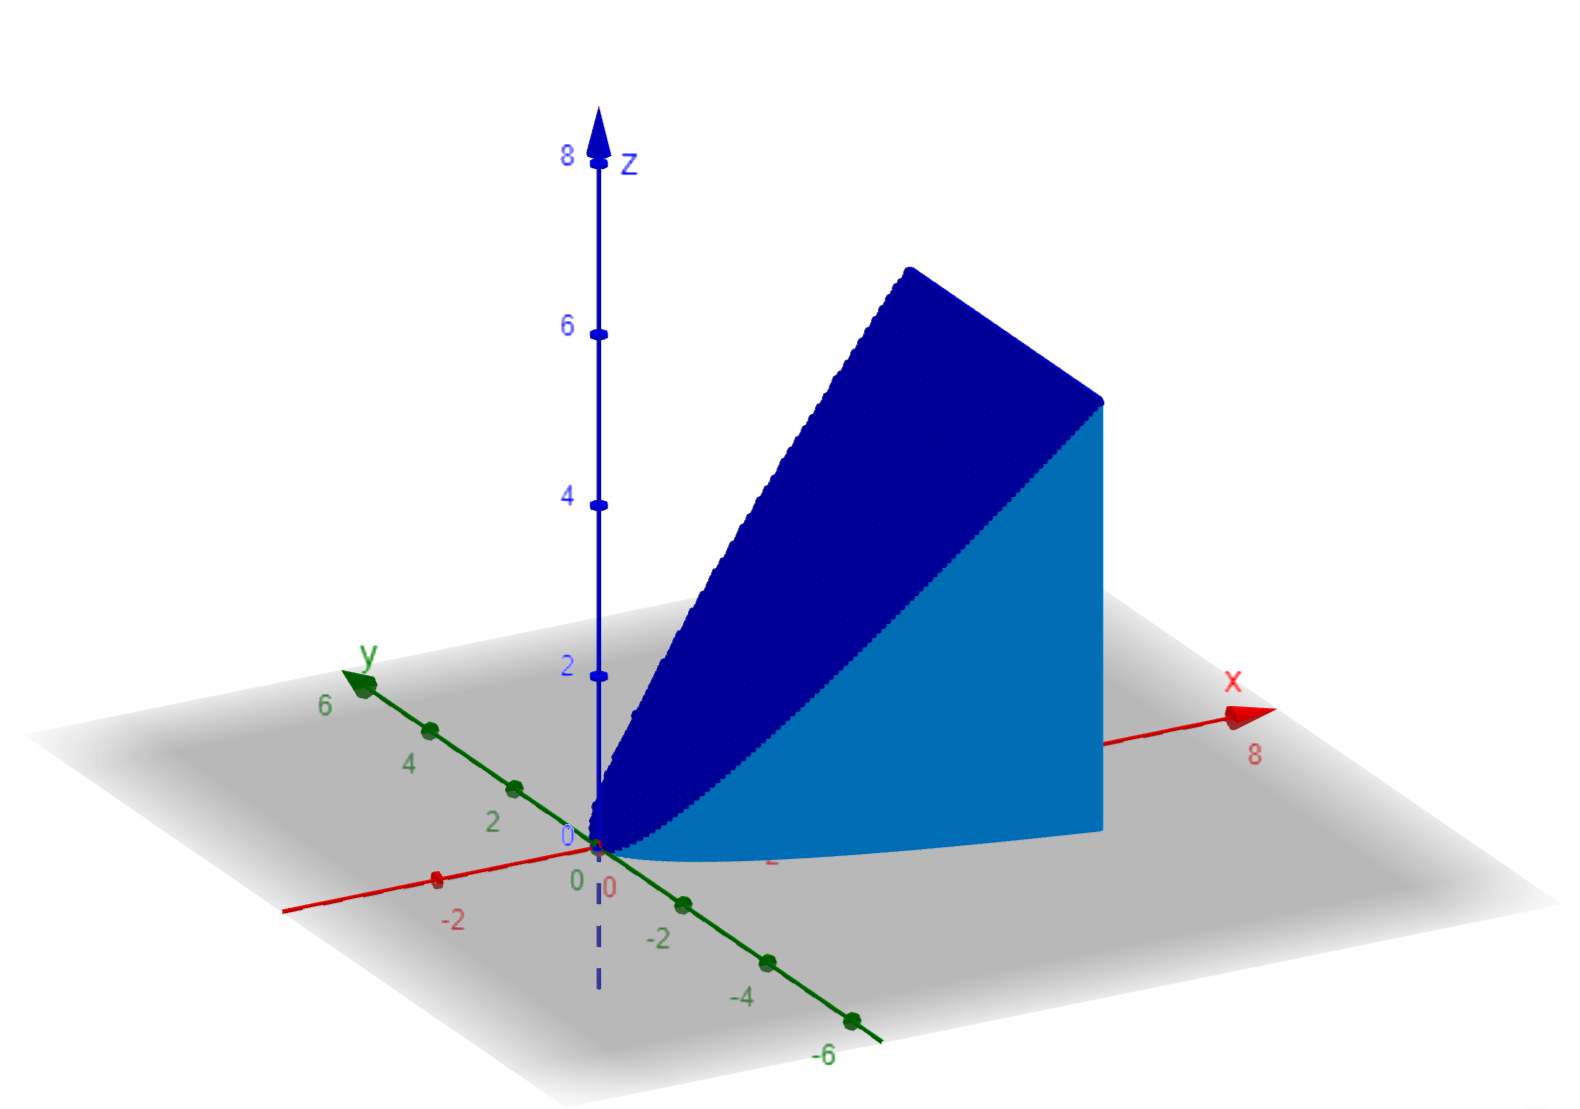
\includegraphics[width=0.7\textwidth]{Pictures/Tutorial 10-1.png} \\
        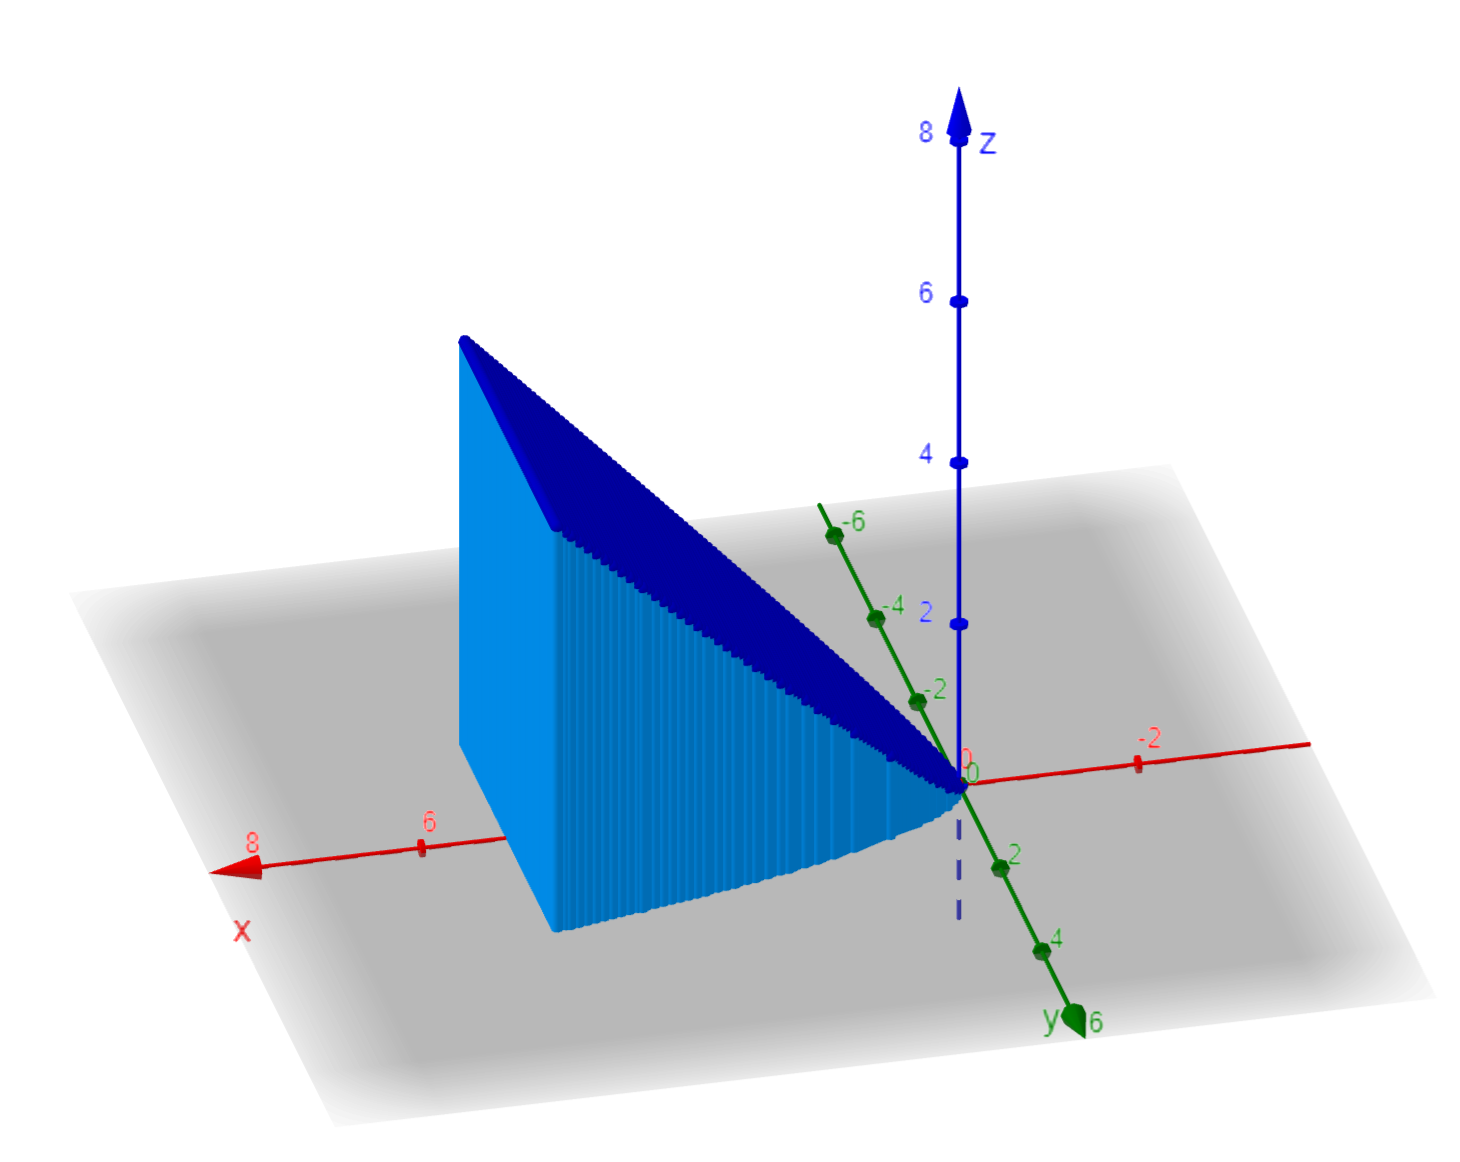
\includegraphics[width=0.7\textwidth]{Pictures/Tutorial 10-2.png}
        \caption{Visualizing the region \(W\) in 3D.}
    \end{figure}
    
    By observation:
    
    The upper bound of \(z\) is given by \(z = x\). 
    The lower bound of \(z\) is given by \(z = 0\). 
    
    The upper bound of \(x\) is found to be \(x = 9\). 
    The upper bound of \(x\) is found to be \(x = y^2\).
    
    The upper bound of \(y\) is found to be \(y = 3\).
    The upper bound of \(y\) is found to be \(y = -3\).
    
    The bounds of our integral should therefore be:
    \begin{align}
        0 \leq & \ z \leq x & y^2 \leq & \ x \leq 9 & -3 \leq & \ y \leq 3
    \end{align}
    
    Other bounds (with different integration orders) may also be correct.
    
    Then:
    \begin{align*}
        \iint_{S} \vb{F} \cdot d\vb{S} &= \iiint_W 1 + 8y \ dV \\
        &= \int_{-3}^3 \int_{y^2}^9 \int_0^x 1 + 8y \ dzdxdy \\
        &= \int_{-3}^3 \int_{y^2}^9 (1 + 8y) z \Big|_{z = 0}^{z = x} \ dxdy \\
        &= \int_{-3}^3 \int_{y^2}^9 (1 + 8y) x \ dxdy \\
        &= \int_{-3}^3 (1 + 8y) \frac{x^2}{2} \Biggr|_{x = y^2}^{x = 9} \ dy \\
        &= \int_{-3}^3 (1 + 8y) \left(\frac{9^2}{2} - \frac{y^4}{2}\right) \ dy \\
        &= \int_{-3}^3 \left(\frac{81}{2} - \frac{y^4}{2}\right) + 8y\left(\frac{81}{2} - \frac{y^4}{2}\right) \ dy \\
        &= \int_{-3}^3 \frac{81}{2} - \frac{y^4}{2} + 324y - 4y^5 \ dy \\
        &= \left(\frac{81y}{2} - \frac{y^5}{10} + 162y^2 - \frac{2y^6}{3}\right) \Biggr|_{-3}^3 \\
        &= 243 - \frac{243}{5}
    \end{align*}
\end{solution}

\begin{tcolorbox}[
        title={Problem 16},
        valign=center,
        nobeforeafter,
        colframe=gray!95!black
    ]
    Evaluate the surface integral:
    \begin{align}
        \iint_{S} \vb{F} \cdot \vb{n} \ dA
    \end{align}
    where \(\vb{F}(x, y, z) = \vb{i} + \vb{j} + z(x^2 + y^2)^2\vb{k}\) and \(S\) is the surface of the cylinder \(x^2 + y^2 \leq 1\) with \(0 \leq z \leq 1\).
\end{tcolorbox}

\begin{solution}
    Rather than computing the flux of \(\vb{F}\) through the three sides of the cylinder, we may compute the volume integral of \(\nabla \cdot \vb{F}\) over the region \(W\) bounded by the cylinder using the Divergence Theorem.
    
    Recall the Divergence Theorem:
    \begin{align}
        \iint_S \vb{F} \cdot d\vb{S} &= \iiint_W \nabla \cdot \vb{F} \ dV
    \end{align}
    
    Then the surface integral is given by:
    \begin{align*}
        \iint_{S} \vb{F} \cdot \vb{n} \ dA &= \iiint_W \nabla \cdot \vb{F} \ dV \\
        &= \iiint_W \nabla \cdot (1, 1, z(x^2 + y^2)^2) \ dV \\
        &= \iiint_W 0 + 0 + (x^2 + y^2)^2 \ dV \\
        &= \iiint_W (x^2 + y^2)^2 \ dV 
    \end{align*}
    
    Recall cylindrical coordinates:
    \begin{align}
        x^2 + y^2 &= r^2 & dV &= r \ dr d\theta dz
    \end{align}
    
    Then:
    \begin{align*}
        \iint_{S} \vb{F} \cdot \vb{n} \ dA &= \iiint_W (x^2 + y^2)^2 \ dV \\
        &= \int_0^1 \int_0^{2\pi} \int_0^1 (r^2)^2 r \ dr d\theta dz \\
        &= \int_0^1 r^5 \ dr \int_0^{2\pi} d\theta \int_0^1 dz \\
        &= \frac{r^6}{6} \Biggr|_0^1 \int_0^{2\pi} d\theta \int_0^1 dz \\
        &= \frac{1}{6} (2\pi) (1) \\
        &= \frac{\pi}{3}
    \end{align*}
\end{solution}


\vspace{1cm}
\begin{center}
    Good luck on your finals :)
\end{center}

\end{document}
